% Modified template

\documentclass{finalyearproject}
\usepackage{url, graphicx,parskip,appendix,float}
\usepackage{geometry}
 \geometry{
 a4paper,
 total={210mm,297mm},
 left=20mm,
 right=20mm,
 top=15mm,
 bottom=20mm,
 }

%Import the natbib package and sets a bibliography  and citation styles
\usepackage[utf8]{inputenc}
\usepackage[english]{babel}
\usepackage[biblabel]{cite}
\usepackage[numbers]{natbib}
\usepackage{tabularx}
\newcolumntype{b}{X}
\newcolumntype{s}{>{\hsize=.3\hsize}X}

\usepackage[ruled] {algorithm2e}
\usepackage{url,amsmath,amssymb,fancybox,listings,pdfpages,caption,multicol,datetime,rotating, booktabs}
%\usepackage[usenames,dvipsnames]{color}
\usepackage{listings}
\usepackage[pagebackref=false,pdffitwindow=true]{hyperref}

%NOTE: The hyperref usepackage should be the last \usepackage!!
%NOTE: When pagebackref=true an error will appear at the end of compiling. press `q' to ignore
%NOTE: Referencing Algorithms does not work if this usepackage is before the hyperref include.!!
%NOTE: This is a comment, ignored when the document is compiled
%NOTE: The following document configuration settings generally do not need to be modified
%NOTE: More packages may need to be added to provide additional functionality

\hypersetup{
    pdftitle    = {Football Match Prediction Application - SureThing},
    pdfauthor   = {Marina Shchukina},
    pdfsubject  = {Subject Area},
    pdfkeywords = {Comma separated list of keywords},
    colorlinks  = true, anchorcolor = blue, filecolor = blue, urlcolor = blue,
    linkcolor   = blue,    %NOTE: change (blue) to (colIdentifier) to have links within the document in Black
    citecolor   = blue,    %NOTE: change (blue) to (colIdentifier) to have citation links within the document in Black
}

\definecolor{colBackGrnd}{rgb}{1,1,0.8}
\definecolor{colKeys}{rgb}{0,0,1}
\definecolor{colIdentifier}{rgb}{0,0,0}
\definecolor{colComments}{rgb}{0,.5,0}
\definecolor{colString}{rgb}{0,0,1}
\definecolor{colWhite}{rgb}{1,1,1}

\newcommand{\MyHookSign}{\hbox{\ensuremath\hookleftarrow}}

\newtheorem{Theorem}{Theorem}
\newtheorem{Proposition}[Theorem]{Proposition}
\newtheorem{Lemma}[Theorem]{Lemma}
\newtheorem{Proof}[Theorem]{Proof}
\newtheorem{Remark}[Theorem]{Remark}
\newtheorem{Claim}[Theorem]{Claim}
\newtheorem{Example}[Theorem]{Example}
\newtheorem{Definition}[Theorem]{Definition}

%NOTE: Setup for including program listings
\lstset{%
    float=H,
    basicstyle=\ttfamily\footnotesize,
    identifierstyle=\color{colIdentifier},
    keywordstyle=\color{colIdentifier}, %
    stringstyle=\color{colIdentifier},
    commentstyle=\color{colIdentifier}, %
    columns=flexible,
    tabsize=2,
    frame=single,
    extendedchars=true, %
    showspaces=false,
    showstringspaces=false,
    numbers=left, %
    numberstyle=\footnotesize,
    breaklines=true,
    prebreak={\space\MyHookSign},
    language=Java,
    backgroundcolor=\color{colBackGrnd},
    breakautoindent=true, %
    captionpos=b%
} %\hypersetup{colorlinks=true, citecolor=\color{colIdentifier}}
\renewcommand{\baselinestretch}{1.5}
\setcounter{secnumdepth}{3}
\setcounter{tocdepth}{3}
\sloppy %NOTE: To ensure the Right Hand Margin is used (Especially for long URLS)
\setlength{\parindent}{0cm}
\setlength{\parskip}{1em}

%NOTE: END of the document configuration settings

\begin{document}

\newcommand{\todo}[1]{\textcolor{red}{#1}}

\DeclareGraphicsExtensions{.jpg,.png,.gif,.pdf}
%NOTE: When inserting Figures if the extension of the graphic file is not provided LaTeX will automatically search
% for the extensions declared above, in the order declared.

\title{\huge{Football Match Prediction Web Application - SureThing}}
\author{Marina Shchukina}
\date{\today}
\degreetitle{Computer Science} % 
\rpttype{BSc (Hons)}    % Replace MSc with BSc for Honours Degree Year projects.
\principaladviser{Dr. Robert McDermott, Dr. Richard Glassey}

\beforeabstract
\prefacesection{Abstract}
The aim of the project is to build a web application simulating the football betting experience and addressing two main issues. Firstly, filling an existing void for a system that makes football match prediction customisable and transparent to the user. For each upcoming match, the application will provide the user with a probability of either of the two teams winning the match based on the current football statistics and expressed in percentage. The user would then be able to influence this probability value by adjusting the weights for each of the several factors that contributed to that result. Depending on the values of the weights, prediction may be different for different users. In the long run, users of the web application would be able to create their own "betting system" by constantly re-adjusting the default prediction weights and hopefully coming up with a set of weights that works the best. Secondly, allowing the users to analyse their past performance and compare their results and prediction weights with the other users of the application.

The stated above would be achieved by taking several steps. First, the background research will be carried out. On completion of the research, 
current similar websites will be researched and a set of requirements will be created to assess users’ needs. After that a layout and overall design of the application will be produced, as well as the desired behavior of its features. Once the prototyping is completed, the main project deliverable, i.e. working web application will be developed and throughly tested. 

\prefacesection{Acknowledgements}
I would like to acknowledge and extent my gratitude to the following people who have made the completion of this project possible:

Dr. Roger McDermott for his support and guidance in this project
Dr. Richard Glassey for his initial help and valueable advice
My husband Murray and baby daughter Scarlett Mary for their support and patience.

\afterpreface 
\afterabstract


%NOTE: Include the relative reference for each chapter to be included
% dividing the thesis file structure into a number of directories aids development
% format: directoryName/filename (the .tex extension is not required for the filename)
\tableofcontents  %NOTE: Will generate a list of Program Listings in the Table of Contents Section

\chapter{Introduction}
\pagenumbering{arabic} \setcounter{page}{1}

A short paragraph introducing the topic the chapter examines.


\section{Background}

A number of pages about the background of the project.

\section{About this Thesis}
This is the thesis of \emph{Insert Full Name Here}, submitted as part of the requirements for the degree of MSc Computing: Software Technology at the School of Computing, Robert Gordon University, Scotland.

A number of paragraphs detailing the main expectations of this body of work.

\section{Problem Areas}
The main challenges associated with the project are:

\section{Report Structure}
A short conclusion summarising the chapter.

\chapter{Background studies and objectives}
\label{ch:Background}

In this chapter the background of the project will be discussed. The chapter will take the reader through the history of sports betting with a particular focus on online gambling. The primary and the extended objectives of the project will be outlined and the professional considerations will be addressed. 

!!!For this chapter put lots of references (especially in the BG subchapter)

\section{History And General Information}
\label{sec:history}
Gambling is nothing new. Since time began, people have been betting on the outcome of an event, be that the victor in a gladiator competition, the winning team in a football match, or the first horse past the finishing post.


\section{Objectives}
\label{sec:objectives}

People have always been interested in games with the element of luck and therefore gambling is one of the oldest forms of entertainment of mankind. The rise of the Internet and mobile devices has made remote gambling more available for a wide variety of users. The reason for that could be that Internet applications and websites can be are easily accessed 24/7. Amongst the most popular types of online gambling can be found card games, dice games, electronic games (such as poker), betting on sporting events, etc.
Sports betting is no longer associated solely with horse racing. Among all types of sports gambling, football gambling is a leading industry with a share about 70% and half a million people betting weekly all over the world.
When it comes to any sports betting (football betting including), the user is trying to predict the result of the event and placing the money on the outcome. This prediction can be made based on a “hunch” or by using logic and domain knowledge, in a lot of cases by both combined. Naturally, this gave rise to a vari- ety of betting software systems that are attempting to predict the next match re- sult. Most of the time those betting systems work as a “black box” not allowing the user to influence the prediction output and preventing the user from understand- ing the exact logic used inside the system.
Football punter can have various strategies when making a betting decision. As mentioned above, the user can buy a prediction software and simply follow the tips suggested by that system. Another option is to make a decision influenced by the opinion of the other tipsters, experts’ opinions or rumours. However, if the aim is to achieve sustainable profit (or minimise the loss from betting) , most experienced punters would ignore betting tips and predictions of others and go for the pure facts trying to make their own prediction. To make this happen, the punter has to aggregate several pieces of information from various sources. This action has to be repeated for every single match.
From my experience, the necessity to repeat an action many times could lead to a creation of interesting software solutions. That is how I got inspired to create an application that would aggregate this information for the user and therefore act as an interactive decision supporting system.

\subsection{Primary Objectives}
\label{sec:primaryobjectives}
The purpose of my final year project is to create a web application that can help users to predict football match results and make profitable bets. There are many similar websites and applications. However, I think my application is different from the other ones. The key feature of the app is the fact that the prediction output is transparent to the user and can be easily adjusted and customised. 


\subsection{Extended Objectives}
\label{sec:extendedobjectives}
Hello!!


The purpose of my final year project is to create a web application that can help users to predict football match results and make profitable bets. There are many similar websites and applications. However, I think my application is different from the other ones. The key feature of the app is the fact that the prediction output is transparent to the user and can be easily adjusted and customised. 

\section{Problem Specification}
\label{sec:projscpec}


\subsection{Limitations and Evaluations}
\label{sec:limiteval}
Hello!!

\section{Social, legal and ethical issues}
Legal
Finding free API for a newly created betting application may become a non-trivial task. Therefore, I am considering using “web scraping” as one of the options to load most recent football data into the system. It can be said that there is a fine line between collecting information using the “web scraping” technique and stealing it. Most of the websites have a copyright disclosure defining the rules for the use of the information they provide. Thus, I will carefully read the disclosure statements and follow them along legally and ethically. 

Ethical
Due to the nature of the application it is inevitable that it will store some basic user data in its database. The application must take all the necessary precautions to protect the stored data and sensitive information. The application will not disclose personal data of its users to any third parties.

Social
There are several advantages of using the application for a rational punter. First, the use of it will hopefully lead to more profitable football betting and also reduce the amount of thoughtless bets. Secondly, the use of application will save time spent on gathering information before making a betting decision.

Professional
Although the main aim of the application is to provide transparent prediction to the user, there is still certain amount of calculation happening in the background. I assume that user will trust the betting system when making a betting decision. Therefore ensuring the accuracy of the calculations and providing  good test coverage is a very important part of the application development.

Hello!!
a wee summary: what we discussed in this chapter
In this chapter we discussed the history. I also introduced the objectives of this paper and lined up several use cases making clear for the user how the application is going to work.

In general, the application is not aimed to promote gambling. Moreover, it supports a more sensible and measured approach to football betting.
In this chapter we discussed…(the main conclusion for the chapter)





\chapter{Requirement Analysis and Specification}
\label{ch:requirementanalysis}
Before designing a piece of software, it is important to hold good understanding of what the final product is supposed to do. During the requirements analysis phase, a number of steps were taken previously to producing a final list of requirements. First of all, a target audience questionnaire was produced and sent out to the potential application users. The results of the survey were then compiled and analysed. Secondly, a number of existing websites that could at least partly solve the problem outlined in the ”Problem Statement” \ref{sec:problemstatement_intro}  were examined and evaluated. Finally, a list of functional and non-functional requirements covering all the aspects of the future web application was developed and documented in this report.

\section{Target Audience Questionnaire}
\label{sec:targetaudiencequestionnaire_req}
The target audience research aims to gather information on the way football punters make their betting decisions. Questions were specifically tailored to find out what kind of content would appeal to the potential users of the application \ref{sec:targetaudience_intro}. Due to the spread of target users, an online questionnaire was used to collect the answers. There were only 9 respondents due to the specifity of the topic. A full break down of the questions asked and the answers received can be found in the appendices \ref{ch:questionnaire_appendix}.

\begin{figure}[H]
	\begin{center}
		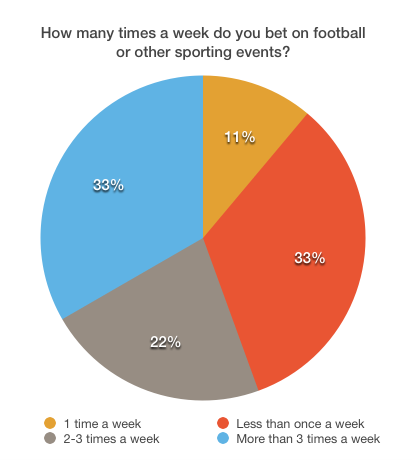
\includegraphics[width=.50\columnwidth]{req/images/howMuchDoYouBet.png}
		\caption{A pie chart illustrating the answers of the questionnaire respondents when asked how many times a week do they bet.} \label{fig:using:howmuchdoyoubet}
	\end{center}
\end{figure}

As it can be seen from figure \ref{fig:using:howmuchdoyoubet}, most of the survey participants are active punters, with the number of placed bets 2 or more per week. 

\begin{figure}[H]
	\begin{center}
		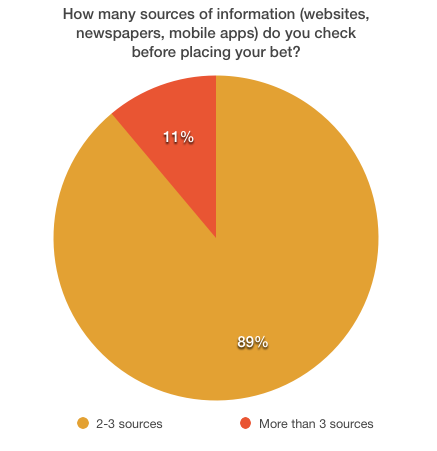
\includegraphics[width=.50\columnwidth]{req/images/howManySources.png}
		\caption{A pie chart displaying the answers of the respondents when asked how many sources of information (websites, newspapers, mobile apps) do they check before placing a bet.} 
		\label{fig:using:howmanysources}
	\end{center}
\end{figure}

\begin{figure}[H]
	\begin{center}
		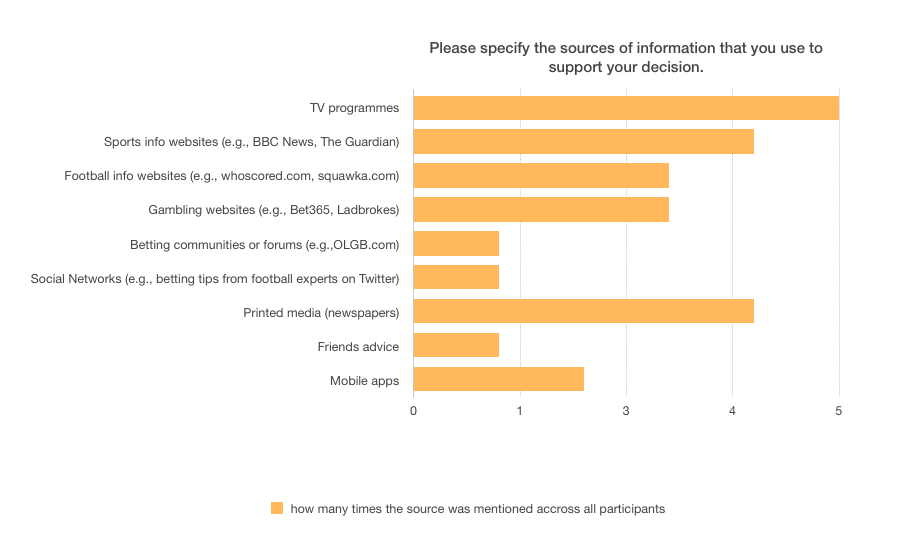
\includegraphics[width=1.0\columnwidth]{req/images/listTheSources.png}
		\caption{A bar chart illustrating the answers of the respondents when asked to specify the sources of information that they use to support a betting decision.} 
		\label{fig:using:llistthesources}
	\end{center}
\end{figure}

Charts in figures \ref{fig:using:howmanysources} and \ref{fig:using:llistthesources} demonstrate that punters tend to analyse data from several sources before placing their bets. This proves a need for an application that can reduce the amount of time people spend switching between different type of media to obtain all the information they need. Among the most popular sources were mentioned TV programmes, sports info websites and newspapers.

\begin{figure}[H]
	\begin{center}
		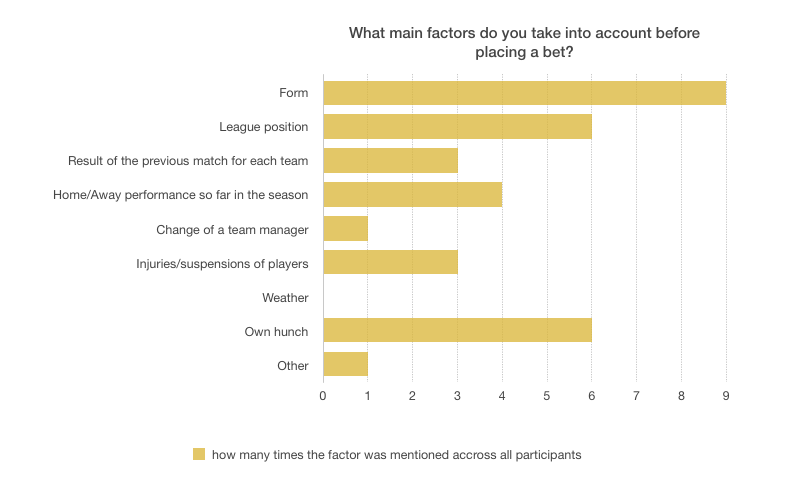
\includegraphics[width=1.0\columnwidth]{req/images/listYourFactors.png}
		\caption{A bar chart illustrating the answers of the respondents when asked to specify the factors they consider before placing a bet.} 
		\label{fig:using:listyourfactors}
	\end{center}
\end{figure}

The respondents were asked to list all the factors that they take into consideration before making a betting decision. They were provided with a long list to choose from and asked to specify their own factors if needed. The bar chart in figure \ref{fig:using:listyourfactors} illustrates the answers. Three factors appeared to be clear winners: form, league position and home/away performance. An interesting point is that punters often use inuition in the decision-making process, as 66\% of the respondents mentioned "own hunch" as one of the factors. Incorporating user hunch into the prediction formula will be a clear challenge for me as a developer, however, it looks like the potential application users would like to be able to include it into the calculation. 

It was expected that more respondents will mention home/away performance as one of the top influences in making betting decisions. The relatively low interest in this factor can be possibly explained by the fact that the value representing home/away performance cannot be simply found in a league table, and a punter needs to make an extra effort to calculate it.

One of the respondents specified an own factor in the field "other": "whether or not the odds appear to offer good value". Considering that most survey participants mentioned that they only use one favourite betting provider when placing a bet, this seems to be an interesting point. It looks like the future application will benefit from offering its users odds comparison and possibly a recommendation, such as "odds of the day".

Another interesting fact is that 100\% of the respondents answered "no" when asked whether they track their betting performance. The answers prove that monitoring performance seems like an extra step for the majority of punters. This observation led me to an idea to consider including a tracking tool into the application. 

Finally, most of the survey participants answered "yes" when asked whether they would find useful a "web application allowing you to participate in the prediction of a match result by making up you own prediction formula".  

Despite the limited amount of respondents, the answers collected with the questionnaire appeared to be a very valuable input to the phase of the project planning.

\section{Researching Current Solutions}
\label{sec:currentsolutions_req}
Before gathering the project requirements, it is good practice to conduct research on what current websites are already available to football fans with interest in betting. The research can be a source of inspiration and could also help to avoid potential design mistakes. During the analysis, it is important to attempt to understand the main purpose of the analysed websites, as well as the way they present information to the user and communicate with them. 

This section is concerned with websites that can be useful for predicting football results. In our context, these are the various online sources of information a football punter would turn to before making a betting decision unless the decision is based solely on intuition. In general, several different types of such websites can be found online, namely:
		
\begin{enumerate}
	\item Sports news websites
	\item Football statistics websites
	\item Bookmakers websites 
	\item Communities for sports fans
	\item "Black-box" prediction applications
\end{enumerate}

This section of the report looks at one or two examples of each of the categories presented above, analysing the weak and strong points of the chosen website and discussing usefulness of the whole category from the point of view of a football punter.
	
\subsection{Sports news websites}
\label{subsec:sportsnewswebsites_req}
This category represents football news websites. Into this category fall both general sports websites with a football section and football news websites, such as:
	
\begin{itemize}
	 \item BBC Sport \citep{source:bbcsport}
	 \item The Guardian Sport News \citep{source:guardiansport}
	 \item Sky Sports \citep{source:skysports}
	 \item The Times Sport section \citep{source:thetimes}
	 \item Football365.com \citep{source:football365}
	 \item Goal.com \citep{source:goal}
\end{itemize}

The sports news websites aim to present the news alongside the essential football statistics. The information is usually not as detailed as on the football stats websites, however the very latest football news compensates for this drawback. Each of the \emph{news} websites named above (BBC News, The Guardian, Sky Sports) have a football section that presents the reader with the combination of football news and stats.  One of the most popular football news websites is BBC Sport Football.
	
\subsubsection{BBC Sport Football}
\label{subsubsec:bbcsportfootball_req}
BBC Sport Football is a very good quality sports news website. It offers a very neat and simple interface and does not overwhelm the reader with irrelevant graphics. Although, it almost looks too minimalistic, the user can still get all the most important information about football teams and players. The website provides authomatically updated live scores accross all featured football leagues.

BBC Sport has a very impressive news coverage of both major and minor British football leagues, as well as the main european leagues. It can also take pride in high quality writers (journalists) contributing to the website. An interesting feature is videos embedded in the webpage.

As already mentioned above, the main drawback is that the stats are kept to a bare minimum. This can be a problem for a serious football fan that wants to analyse the details of the game from all possible angles. However, for the purpose of a punter this level of statistics should be sufficient.
	
\begin{figure}[H]
	\begin{center}
		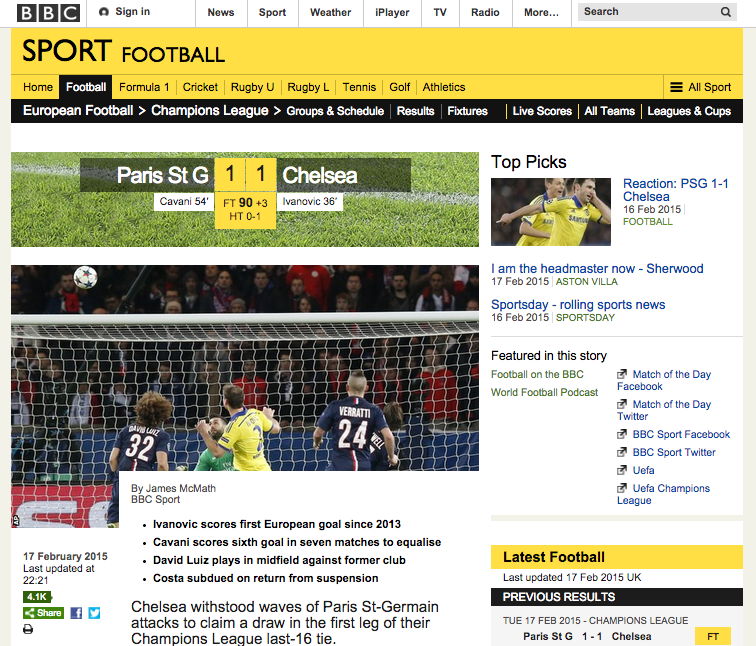
\includegraphics[width=.80\linewidth,natwidth=610,natheight=642]{req/images/bbcsport.png}
		\caption{BBC Sport - Football section} \label{fig:using:bbcsport}
	\end{center}
\end{figure}
		
\subsection{Football statistics websites}
\label{subsec:footballstatswebsites_req}
There can be found a large selection of football statistics websites focusing on detailed stats and analysis on football matches, teams and players. These are some examples of websites in this category:
			
\begin{itemize}
	\item WhoScored \citep{source:whoscored}  
	\item Squawka  \citep{source:squawka}
	\item Injuries And Suspensions \citep{source:injuriesandsuspensions}
\end{itemize}

\subsubsection{WhoScored}
\label{subsubsec:whoscored_req}
Among all the football stats websites I have analysed, WhoScored is one of the most impressive ones. It has a lot of statistics, but most of it seems to be quite relevant. The website is extremely well designed, and its navigation is intuitive. WhoScored offers statistics and deep analysis on the major European divisions, as well as providing data on over 500 leagues and 15,000 teams. As to the data source, the website is supported by Opta, the largest and a very reliable live sports data company that stands behind BBC Sport, Sky Sports and other significant UK sports news providers.

The way "WhoScored" presents information on particular matches, both upcoming and played, is detailed while being uncluttered,which makes it both very useful and easy to use. This is definitely an aim of this particular project and I will be using a similar format when designing the website. 

\subsubsection{Squawka}
\label{subsubsec:squawka_req}	
Squawka is another website worth looking at. 
		
\begin{figure}[H]
	\begin{center}
		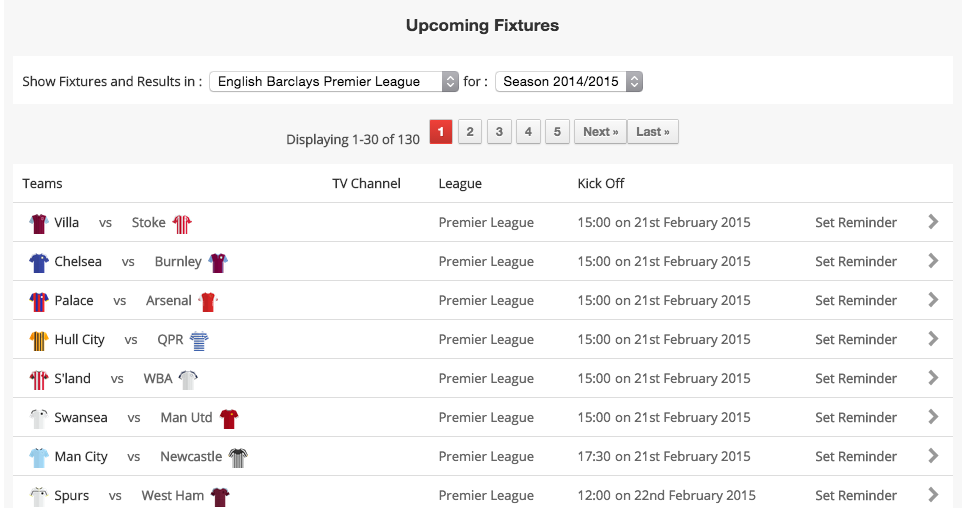
\includegraphics[width=.80\linewidth,natwidth=610,natheight=642]{req/images/squawka.png}
		\caption{Squawka} \label{fig:using:squawka}
	\end{center}
\end{figure}
	
It is an application for football fans that uses real-time data visualisations to explain the game. The main idea behind it is to show users the live stats as the game is being played. 

From a visual point of view, Squawka has a nicely designed, pleasant interface. However, it is a little bit heavy on the client-side (Javascript), which contributes to sometimes slow performance. Another downside of the website is an extensive amount of adverts that distracts the user form the main content.
	
\subsection{Bookmakers Websites}
\label{subsec:bookmakerswebsites_req}
	
With the arrival of the Internet many existing bookmakers opened up web based operations to complement their existing business. Within short period of time online gambling became very popular with punters all around the world. Most online bookmakers contain high quality sports statistics that aims to support users' betting decisions.

Names like Ladbrokes, Bet365, William Hill are probably one of the most popular bookmakers online.

\begin{itemize}
	\item Paddy Power \citep{source:paddypower}
	\item Ladbrokes \citep{source:ladbrokes}
	\item Bet365 \citep{source:bet365}
	\item William Hill \citep{source:williamhill}
\end{itemize}

\subsubsection{Bet365}
\label{susubsec:bet365}

According to the \citet{wiki:bet365}, "Bet 365 Group Limited, is a United Kingdom based gambling company. Bet365 is one of the world’s leading online gambling groups with over 14 million customers in two hundred countries". In my opinion, Bet365 has one of the nicest websites among bookmakers. The website is very well structured, it has intuitive, user-friendly navigation and is easy to use. Bet365 offers a free live streaming service and an impressive coverage of live sports statistics.

\subsection{Communities for sports fans}
\label{subsec:communities_req}
Communities is a category of websites with an interesting idea behind it. These websites are specialised social networks for sports fans and punters. So far, websites of this type are not particularly popular, maybe because gambling is more of an individual pursuit.

Many of the features of websites in this category, such as experts tips, users' comments, forums, can be very useful from a punter's perspective, especially when dealing with a league you are not overly familiar with. I have analysed three websites in this category.
	
\begin{itemize}
	\item OLGB Betting Community - \citep{source:olgb}
	\item Vital Football News and Fans community - \citep{source:vitalfootball}
	\item Punters Lounge - \citep{source:punterslounge}
\end{itemize}

OLGB is a friendly community for punters with many interesting features and tools. It will be analysed in more detail in a separate subsection below. Vital Football is a "network" website. It runs a separate website for every football club from the Premier League and the Football League in England and the Scottish Premier League with each "club site" having their home page, own editors and a forum. Punters Lounge is a "betting and poker community". Its most interesting feature is a forum for sports punters. The website also offers free betting advice tips, live sports streaming and odds comparison.
	
\subsection{OLGB Betting Community}
\label{subsec:olgb_req}
OLGB community market themselves as a website for punters who share their expertise and work together to maximise their betting profit, so it is very relevant to this project. OLGB has a wide variety of features and tools. However, real punters' opinion and tips is the main focus of this website. For example, the user can navigate to an upcoming event page on OLGB website (in the section "free tips") and check how many other users predicted either team to win. Users' choice is usually justified with an comment. For each option OLGB suggests the best odds from one of the most popular bookies. This saves user the trouble of going to a website like OddsChecker\cite{oddschecker} to compare the odds. The comments feature is very interesting and it can be applied as an "optional requirement" for this project.

OLBG also runs a virtual betting game (tipster competition) where users can "bet" virtual money on real betting events. The tipsters in the top 100 of the tables for each sport each month receive a real money prize. Users of the website can also see a leaderboard of the most successfull tipsters. The leaderboard contains information on the amount of tips made within certain period of time, LSP (Level Strike Profit), ROI (Return on Investment) for each tipster. The virtual betting feature is very relevant to this project. A simplified version of the leaderboard could also be implemented. 

OLGB has more to offer. It is a punter's paradise in a way. For example, there is a betting forum, betting blogs section, betting school and much more. The community website has a tight connection to several popular bookmaker websites. For example, it offers a tool to help users to compare bookmakers websites. It also promotes free bets and various "bookies" promotions.

The website has also several drawbacks. Firstly, the interface looks a little outdated and it takes a while to find your way through the complicated and rather confusing navigation. Secondly, the "Help" section does only answers some questions and can be slightly disorientating for a new user.

\subsection{Black-box prediction applications}
\label{subsec:blackboxapplications_req}
These are betting applications that are being marketed as systems that can predict the outcome of a football match using their own unique statistical models and calculations. Known as black-box systems, these applications avoid sharing the exact logic used inside the system with the user. The punter subscribes to a betting system online and simply follows its suggestions, for example, estimated outcome of a football match, overestimated events that the user should bet on, etc. These are the example apps in this category:

\begin{itemize}
	\item Math Betting \citep{source:mathbetting}
	\item Footbee \citep{source:footbee}
	\item Vitibet \citep{source:vitibet}
	\item Forebet.com - Mathematical Prediction \citep{source:forebet}
\end{itemize}

When paying for the subscription for a black-box betting application, the users assume that they are gaining access to a unique system created by team of experienced football experts. Additionally, there is an expectation that the application has complicated statistical models and calculation analysing a large database of football statistics behind each betting tip. The users also hope that they are paying for a \emph{secret} betting system that is known to and is used by only limited number of other punters. Summing up, a black-box system application sounds like an easy way to sustainable profit. Unfortunately, this does not have to be the case. 

According to \citet{art:simplebettingsystem}, the complexity of a betting system does not necessarily correlate with its profitability. The logic behind a successful betting system can be relatively simple and would still work. Secondly, in order to predict a football match result, it might be enough to analyse only relatively recent events (for example last 6 matches, recent players' performance, etc.), without having to perform computations on large set of historic football data. This is due to the fact that over time many various factors can cause change in team performance. Therefore, analysing data from several months ago would not help the punter to make more precise prediction.

\subsection{Conclusion}
After having analysed the above websites, I came to the following conclusion. A well-chosen combination of several websites would definitely be able to provide enough information to make a thoughtful betting decision.

Many punters have their own football betting system (betting strategy) \cite{art:simplebettingsystem}. Although even the best system cannot guarantee success, it can greatly increase the probability of making a profitable bet. Therefore, before making prediction, a thoughtful punter will conduct a little research for each match. The aim of such research would be to collect relevant information about the teams involved in the game. The type of the information will depend on the \emph{input variables} of the betting system used by this particular punter. The problem is that many football stats websites overwhelm their users with detailed statistics that is irrelevant for prediction purposes. Hence, punters often have to "hand-pick" the important information from several sources for each match. 
 	
The developed application will attempt to put all the relevant statistics in one place and break the information down into logical modules. In addition, the application will enable users to pick the input variables and assign them a weight of user's choice, representing the importance of the input variable for the match results prediction.
 
\section{Requirements Specification}
\label{sec:requirements_req}
 \citet{book:radice1998software} define project requirement as follows: "A \emph{requirement} conveys an essential property that the system must or should satisfy." Requirements analysis involves gathering information in order to meet customer needs and defining what the future application is expected to do. 
This phase of software engineering is especially important in the industrial environment, when developing an application for a customer. In that case, clarifying the requirements in the early stages of the project would help to ensure that both sides understand and agree on the feature set of the future application. 

Although it is not very likely that requirements for this project will change during the development process, defining requirements can be very beneficial. The detailed requirements analysis will aid understanding how different parts of the project are expected to interact with each other, as well as how the application will communicate with its users.

For better transparency project requirements have been split into functional and non-functional requirements. Functional requirements will be further subdivided into mandatory and optional, depending on the degree of constraints.

Before outlining project requirements, I would like to start with some definitions relevant to the project as a whole.

\subsection{Definitions}
\label{subsec:definitions_req}
\textbf{Application Football League} - in order to reduce unnecessary complexity at this stage of the project, the application will be only supporting one league.

\textbf{Matches Overview} – a list of upcoming and played matches presented on the main page of the website.

\textbf{Dashboard} - an interface available to authorised users. Dashboard is a starting point for users to view, edit and commit saved matches, as well as access other prediction-related content and tools.

\textbf{Prediction Module} – my own term. Each prediction module represents an input system variable in the betting system    
 \citep{art:bettingsystemvariableparameters}. The aim of each prediction module is to evaluate and compare in a predefined way blocks of latest football statistics for each of the teams participating in the game (for example, position of each team in the league standings table). The result of this comparison is a module \emph{prediction value} that expresses the probability of either team to win based on one module statistics.

\textbf{Prediction Settings} - a set of weights assigned to prediction values in the betting system in order to forecast the result of the match.

\textbf{System Default Prediction Settings} - application has a set of "recommended" weights that are used in the prediction calculation by default. 
 
\textbf{User Default Prediction Settings} - each user of the application can override the system default prediction settings and save their own set of weights. From the moment those weights are in the database, they will be applied by default in the prediction calculation for each match saved by the user. 

\textbf{Match Specific Prediction Settings} - each user of the application can also save a set of prediction settings applying to only one match. 

\textbf{Match result} - "Home Win" in case of the win of the hometeam, "Away Win" in case of the win of the awayteam, "Draw" for the draw.

\subsection{Functional Requirements}
\label{sec:functionalrequirements_req}
Functional requirements describe the behaviour of the application in terms of its functionality. These are the "must have" functions of the application addressing the business targets that application must satisfy. Good functional requirements must be complete, coherent and unambiguous.
 
In order to add structure to the design and development process, the project was logically divided into high level features of the future application. The \emph{mandatory} functional requirements are grouped by the functionality related to these features.

\subsubsection{Authentication and User Profile}
\label{sec:authandprofile_req}
These are the requirements for the basic functionality of the web application, such as account registration, login, logout and account management. The requirements relating to the user profile page will be also listed in this subsection.

\textbf{The application will allow users to register and create a new account with the application.}
\begin{itemize}
  	\item User will be able to register using a standard web form.
  	\item For the registration purposes user will provide a valid email address and a password.
  	\item User will confirm a password in a separate input field.
  	\item On completing the registration form, the application will send the user an email containing a confirmation url.
  	\item On successful confirmation of an email address using the above confirmation url, user will be successfully registered.
  	\item In case of any technical problems with the initial confirmation email, the application will generate a new confirmation url and send it to users on request.
\end{itemize}

\textbf{The application will allow users to sign into their accounts using a standard web form.}
\begin{itemize}
	\item User will provide email address and a password associated with it.
	\item When signing in, user will provide valid credentials, otherwise an application will throw a validation error.
\end{itemize}

\textbf{Account management}
\begin{itemize}
	\item The application will enable users to manage their accounts by changing personal information related to it (for example, location, favourite football team) using a web form.
	\item Users will be able to change the email address associated with their account.
	\item Users will be able to change their passwords at any time.  
	\item The application will provide users with a way to recover their lost passwords.
\end{itemize}

\textbf{User profile}
\begin{itemize}
	\item The application will have a special user profile page containing all the essential information about the current user.
	\item Users will also be able to view profile pages of other users of the application.
\end{itemize}

\subsubsection{Matches Overview}
\label{subsubsec:matchesoverview_req}
Below can be found requirements related to the matches overview.
\begin{itemize}
	\item On the main page of the application, user will be presented with a list of upcoming matches for the current season in the league.
    \item User will be also able to view a list of matches already played in the current season and switch between upcoming and played matches using navigation tabs.
   \item Each of the entries in the match list will contain the most basic information about the match, e.g. names of the teams participating in the event, kick-off time and date, full-time score (only for the played matches).
   \item For each of the unplayed matches, user should be able to navigate to the match page and see more details about the match.
  	\item From the main page user will be able to save any unplayed match to the dashboard for a later review.
  	\item For each of the played matches user will be able to navigate to the match page and see more details about the played match.
\end{itemize}

\subsubsection{Prediction}
\label{subsubsec:prediction_req}
In this part of the report, the Prediction feature of the application will be explained and the related requirements will be listed.

The outcome of a football match will be calculated after evaluating several factors that can influence football match result. An example of such factor could be previous match result, position in the league, team performance at home or away, the recent change in team management, individual performance, as well as injuries and suspensions of team players. When considered as a part of a betting system, factor is basically an \emph{input system variable} \cite{art:simplebettingsystem}. As already mentioned above in the "Definitions" \ref{subsec:definitions_req}, each of those input variables will have a "prediction module" representing it in the application and the main outcome of each prediction module will be a "prediction value", percentage that tells the user which team is more likely to win the match.

Finally, the betting system will assign a weight, a value of which will depend on user settings, to each of the prediction values. The weights or prediction settings determine the relative importance of each factor. By applying the weights, user indicates that some factors are more important to the outcome of this particular game than the others. The final result will be calculated as a weighted average.

As it can be seen from the above explanation, the list of factors that can be considered in the application can be quite long. To simplify the development process, it was decided to limit this list to only three factors. Factors listed below were chosen based on the analysis of the data obtained from the target audience questionnaire \ref{sec:targetaudiencequestionnaire_req}. "League position" and "Form" were two top answers when answering the question

\begin{itemize}
	\item League position of each of the two teams
	\item Form of each of the two teams
	\item Home/Away performance of each of the two teams
\end{itemize}

During the implementation phase these factors will be transformed into prediction modules and integrated into the application. On the top of that, an extra prediction module, "User Hunch" will be created. This is a special module that will allow the users to incorporate their intuition into the prediction calculation and thus influence the result of prediction. "Own Hunch" was also one of the most common responses among the questionnaire participants.

Below can be found the requirements relating to the prediction feature of the application.

\begin{itemize}
  \item To calculate prediction values for each module, application will use \emph{system default} settings in absense of \emph{user default} prediction settings or \emph{match specific} settings.
  \item The application will make use of the \emph{user default} prediction settings (explicitly set by the user using a web form) in absence of \emph{match specific} settings.
  \item The application will apply \emph{match specific} settings in case user has set them for this match.
  \item Match result prediction will be calculated as a weighted average of prediction values using an appropriate set of weights based on the logic outlined above.
\end{itemize}

\subsubsection{Upcoming Match View}
\label{subsubsec:upcomingmatch_req}
For each unplayed match, user should be able to view relevant football statistics, change the match result prediction by adjusting the weights and "commit to bet" the match, once satisfied with the final output. Below can be found the requirements illustrating this part of the application functionality.

\textbf{Functionality available for all users.}
\begin{itemize}
	 \item Upcoming match view will contain general information about the match in the view "header", e.g. names of the teams participating in the event, kick-off time and date, the result of the last match for each of the teams.
    \item As well as the match "header", the view will present the user with a list of prediction modules.
    \item Each prediction module will contain a relevant piece of football statistics.
    \item For each prediction module, it will be clear, which team is more likely to win and what is a probability of this outcome, given that match prediction is based solely on this module. In other words, each prediction module will have its \emph{prediction value} clearly indicated.
    \item In case the user has not saved the upcoming match to the dashboard, the view will display only list of prediction modules and associated prediction values. However, it will not be possible to make match result prediction or commit the match.
   \end{itemize}
   
\textbf{Functionality available for the users who saved the match to the dashboard.}
\begin{itemize}
	\item The user will be able to see what weights are being used for each prediction module.
    \item The application will allow the user to set new match specific prediction weights on this page.
    \item As well as the modules based on the football statistics, the upcoming match view will contain a special module, "user hunch". Its importance was already outlined in the subsection "Prediction" \ref{subsubsec:prediction_req}. 
    \item User will be able to commit the match, once satisfied with the result of the prediction.
    \item Once the match is committed, the prediction cannot be changed.
\end{itemize}

\subsubsection{Played Match View}
\label{subsubsec:playedmatch_req}
After the game has been played, the user will be able to navigate to the played match page. The page will contain brief football statistics as well as the summary of the performance of users who placed the bet. This view should be more about the retrospective analysis of the users' betting strategies, i.e. the weights used for modules, rather than the detailed statistics from the actual match, i.e. shots on target, possession, etc. Hopefully, the information presented in this view will allow users to compare their results with the fellow punters and encourage them to analyse their own betting strategy and optimise performance.

These are the requirements relating to the played match view.

\begin{itemize}
	\item Played match view will have a match "header", similar to the header in the upcoming match view.
	\item User will be able to view a brief summary of football statistics  at the moment of the event. This information will give the users an idea on how the two participating teams were performing previously to the played match. (????)
	\item Users will be able to see an overview of the website population performance, more specifically performance of users, who committed a bet for this match.
	\item Users will be able to see the visualisation of the website population's choice of prediction weights used for this match, possibly a pie chart.
	\item The view will also have the visualisation, possibly a bar chart, of the website population's choice of the winner for this match (hometeam, awayteam or draw). 
	\item It should be clear from the view what was the result of the bet for an authenticated user. The view will clearly indicate the user's choice and prediction probability. This part of the view will be only available for users who bet on this match and ommitted for the rest of the population. 
\end{itemize}

\subsubsection{Dashboard}
\label{subsubsec:dashboard_req}
Dashboard is a key view of the application.

The idea behind the dashboard in this application is similar to online shopping experience: user saves an item to the shopping basket and can later submit a purchase or cancel it. In our case, user browses through the list of matches on the main page of the application and saves matches to the dashboard for a later review. The requirements listed below describe the dashboard functionality in more detail.

\begin{itemize}
    \item User can save a match to the dashboard from the matches overview  \ref{subsubsec:matchesoverview_req}.
    \item User can remove any unplayed or played match from the dashboard.
    \item Dashboard will have a \emph{dashboard menu} holding the links to various tools and views. Suggested entries of this menu are "Upcoming Matches", "Archive", "Prediction Settings".
    \item "Upcoming matches" will be a default view of the Dashboard. It will contain all the saved matches that have not been played yet.
    \item Tab "Archive" will navigate the user to a view containing the saved matches that have already been played.
    \item "Prediction Settings" tab will open a view with a web form, which can be used to save the user default prediction weights.
    \item In the list of saved matches (both upcoming and played), it will be clearly indicated (colourcoded) whether a saved match was committed and what did user predicted.
    \item If there are any committed matches in the Archive view, it will be clearly indicated whether the user won or lost a bet. 
\end{itemize}

\subsubsection{Notifications}
\label{subsubsec:notifications_req}
The system should be able to notify its users whether they won or lost the bet. 
\begin{itemize}
    \item End of a match is what will trigger new notification messages in the application. Once a game is finished (the fill-time score is available), the application will send a notification to the user.
    \item The user will be able to view the list of all notifications.
    \item The user will be able to delete a notification.
    \item The user will be also able possible to delete all notifications from the list.
\end{itemize}

\subsubsection{Leaderboard}
\label{subsubsec:leaderboard_req}
The application will have a Leaderboard, which is a table comparing the current standings of the application users in terms of their bettings performance.
\begin{itemize}
    \item The leaderboard table will display players' usernames, their total win and loss points. The table will be sorted in order of win points.     
	 \item Hence, the most successful punters will be on the top of the table.
\end{itemize}

\subsubsection{Optional requirements}
\label{sec:optional_req}
The functional requirements were split into two main groups: mandatory and optional. This is due to the fact that the application was developed over a relatively short period of time and there was not enough time to implement all of the intended functionality. Mandatory requirements represent the "minimum viable product", a product with the core features. 

On the other hand, the optional requirements illustrate possible improvements that can be made to the application in the future. Additional research will be needed in order to decide which of the features listed bellow will be the most useful for the target users.

\begin{itemize}
    \item The application will implement "Sign In with Facebook" functionality allowing its users to login with a single click.
    \item The application will have more prediction modules. Suggested modules are "Recent change of a team manager", "Injuries and suspensions of players", "Individual players' performance", "Previous game result", etc.
    \item The user will be able to add/remove any prediction module from the Upcoming Match View. This will help keep the focus on only relevant information from the user's point of view.
    \item The application will offer a betting performance tracking tool that will record the details of the past bets and also keep track on whether the punter is profitable in the long run.
    \item The application will offer its users odds comparison functionality. It is a known fact that the odds for the same event may vary greatly between different bookmakers. The application will compare the odds across the most popular bookmakers and suggest the best option with regards to the user's prediction (home win, away win or draw). Clicking on the suggested odds will take the user to the bookmaker's website or open a bet slip.
    \item The application will get some features of a sports fans community. Users will be able to leave comments on each match explaining the prediction they made and also follow each other. Followers will see the comments from the followed users in their news feed. The news feed will be accessible from the dashboard.
\end{itemize}

\subsection{Non-functional Requirements}
\label{sec:nonfunctional_req}
Non-functional requirements specify how the system is going to perform. 

\begin{itemize}
	\item \textbf{Usability} - The application interface should be easy to understand and learn for a new user. The navigation of the website should be highly intuitive.
	\item \textbf{Responsiveness} - The application should be fully responsive. The websites will be tested for a variety of screen resolutions and the minimum screen resolution will be 640x960 (DVGA - iPhone).
	\item \textbf{Performance} - Optimising performance will be crucial for the application, as there is a direct correlation between the application response time and the user experience.  Performace problems will be detected and eliminated as soon as they appear. 
	\item \textbf{Cross-browser support} - The application will be supported on a minimum set of web browsers, such as Chrome, Internet Explorer 9+, Safari, Firefox.
	\item \textbf{Maintainability} - The focus should be on delivering clear and maintainable code. The code needs to be easily understandable by other developers. For this purpose the best practices of software development and the used languages will be utilised throughtout the implementation phase of the project.
	\item \textbf{Extensibility} – The system will be developed with a large-scale application in mind. It should be easy to apply ongoing changes to the project.
\end{itemize}

\section{Overall Architecture}
\label{overallarchitecture_req}
The high level components of this system are quite simple. 

Design of an application a a whole, overall design (just boxes and lines)
Architectural diagram (overview) (aosabook.org/en/moodle.html -example), quite high level


\section{Choice of Third Party API}
\label{sec:thirdpartyapi_req}
	
After analysing the functional requirements, it became apparent that this type of application will need the latest football data in order to operate correctly. The easiest way to load data into the application would be to integrate the application with a third party API. The process of finding an appropriate API for the project will be described in this section. 
	
After a brief research, one thing became apparent. Live football data is a very desirable product and therefore it is not easy to find free of charge live football data API. The key problem is that the data has to be very recent. Real-time data in particular is very expensive, because of its use by the gambling industry for betting on various markets as the games are going on. It is actually much easier to find free historical football data.  
	
This is a (not complete) list of API providers that I researched about.
	
\begin{itemize}
	\item Optasports.com \citep{source:opta}.\par
Opta is an industry leader. It provides a wide range of XML feeds covering many sports. The feeds include fixtures and results, live scores, live player stats and many more. Data provided by Opta is very reliable and is used by top-notch clients, such as BBC Sports, BT Sport, Sky Sports, as well as many betting providers and newspapers.		
	\item Openfooty \citep{source:openfooty}.\par 
	Openfooty is an interesting project with very detailed API documentation. However, a quick look at the developer forums shows a stale community and many questions about why no one seems to actually be able to get a developer key. Unfortunately, I also did not manage to obtain a key for this API.			
	\item Football API \citep{source:footballapi} .\par
This is a paid API service. The API restricts by IP addresses and limit calls based on the package. On the bright side, it offers the English Premier League endpoints for free (demo use). The API includes endponts for competitions, teams, standings, live scores, fixtures and commentaries.	
	\item XML Soccer \citep{source:xmlsoccer}. \par
	Another paid API service that offers full access to the Scottish Premier League data for free.
		
\end{itemize}
	
Football API was chosen to be integrated with the application. As already mentioned in the "Definitions" \ref{subsec:definitions_req}, it was decided to support only one league for the time being. Football API offers its users free access to the English Premier League, which seems to be a great choice for our application, as this league's worldwide popularity will hopefully make it easier to find other league-related data and information that might be needed during the development process.

\section{Project Plan}
\label{projectplan_req}
The project progress timetable is presented in the Gantt diagram below. Two main milestones were set for this project: firstly, to develop the first prototype of the application and secondly, to complete the second prototype by the end of April, 2015 (this includes all the testing and bug fixes). 

The first prototype will have implemented most of the high level features of the application as introduced in the section "Requirements" \ref{sec:requirements_req}. The second prototype is a more refined version of the application; it will implement all mandatory requirements listed above and have the visual side of the website polished up. 


\chapter{Application Prototype}
\label{ch:Prototype}
Before making a start on of the implementation phase, a lot of effort was put into the creation of the application prototype. Prototyping is a process of developing the initial model of the future application in order to determine the correct application structure, its functionality and the general concept. A prototype is just a model and may differ from the final product.

The project requirements outlined in the previous chapter of this report were used in order to create a mind map representing pages of the future application. This helped understanding what exactly is expected to be seen on each page of the website and what is the user journey in terms of the navigation. Wireframes were created for all the pages of the website. For this purpose was used just paper and pencils to aim flexibility.

In terms of the methodology, a hybrid of Agile and the traditional Waterfall approach was used for this project. Speaking of the traditional Waterfall approach, some of planning was made beforehands, for example requirements specifications, use-case diagrams, wireframes, etc. On the other hand, for the whole implementation phase was used test-driven approach that utilises the best of the agile techniques.

In general, Agile methodology focuses on team communication and project transparency. Nevertheless, one of its advantages is an extreme flexibility, therefore most of the basic components of Agile can still be effectively used by a single person. The key feature of the version of Agile adopted for the project was breaking down the project workload into clearly defined units of work (high-level features introduced in the chapter "Requirements Analysis" \ref{ch:requirementanalysis}), each associated with an iteration, and setting a milestone for each of them. Excel sheets were used for defining the set of tasks for each iteration. GitHub issue tracker was also used as a supporting productivity tool for this project. Code related tasks were recorded as "issues" for the project GitHub repository. The GitHub issue tracker appeared to be a very efficient tool for keeping the focus. TDD or test driven develoment was another key Agile technique adopted for the project. The unit tests covering business logic were always written before the implementation and the next sprint has not been started unless all tests from the previous sprint passed. 

In summary, in this section will be described the process of transforming project requirements into the system design. Several design cornerstones (website structure mind map, a set of wireframes) were produced beforehands. Other elements of the application design (use cases, database schema) were updated in iterations, inline with the Agile methodology. 

\section{Application Structure}
\label{sec:applicationstructure_prototype}
The prototyping process started with producing a large mind map of the future application.  I found mindmapping a very useful way to brainstorm on my ideas, capture and organise them. The final version of the diagram puts together the structure of application pages, navigation scenarios and other ideas relevant to the design. A full mind map can be found in the figure below.

\begin{figure}[H]
	\begin{center}
		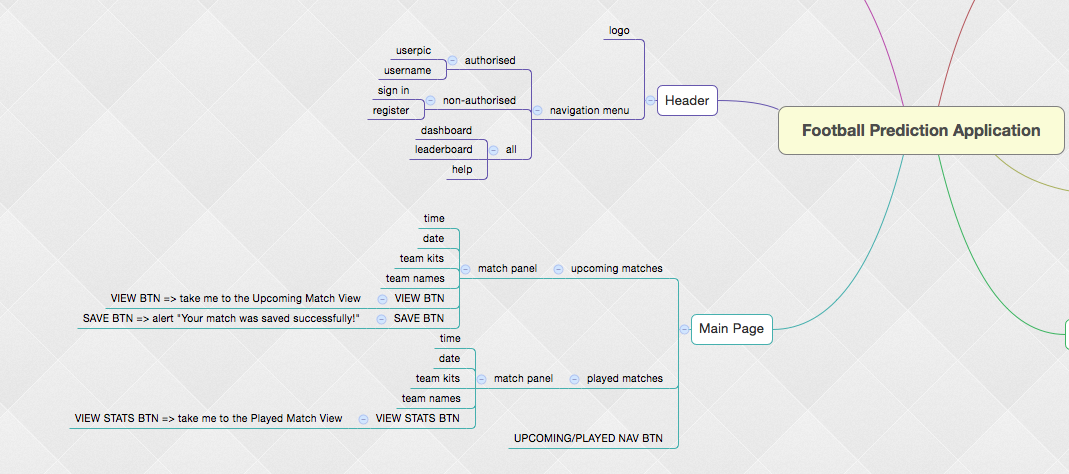
\includegraphics[width=.90\textwidth]{design/images/mindmap}
		\caption{Mind map capturing the result of the initial brainstorming on the application structure and navigation scenarios.} \label{fig:using:mindmap}
	\end{center}
\end{figure}

\section{Inspiration}
\label{sec:inspiration_prototype}
As the next step, I took another look at the currently available websites, hoping to get some ideas on how to approach the visual side of the project and to improve its usability. This step is an important stage of an application prototyping process: it allows to learn from the best design practices and possibly avoid potential errors. The usual practice is to first concentrate on several websites of the direct competition. However, the future application does not really have any direct competitors, as the idea behind the project is quite new. Therefore, I concentrated on the football statistics and news websites (listed in the chapter \ref{ch:Requirements Analysis}, subsection "Current Solutions") making a note of how those websites present football statistics to their users.

\section{Wireframes}
\label{sec:wireframes_prototype}
When speaking about prototyping, in the early stages the first choice of many designers is often a piece of paper and a pencil. Sketching has a number of advantages when compared to the use of the editors, such as Fireworks or Photoshop. When using editors, it is easy to get distracted by brushing up unnecessary details too early. On the opposite side, sketches offer a lot of flexibility. It is easy to add notes, make small changes or replace an outdated sketch with a fresh one.

In case of this project, each of the sketches represented a separate “view” of the website. The scale of a “view” might differ. For example, some sketches show a whole page (home page, dashboard page, etc.), others just showed certain blocks of the website, such as header, footer, user profile container in more detail. I always added a lot of comments to explain the navigation and sometimes expected output. Sketches were one of the most powerful tools I used during the prototyping process. 


Scans of the drawings

\section{Visual Design: Branding, icons, Font}
\label{sec:visdesign_prototype}
First website prototype in a photoshop/Fireworks
Early prototype using html and css, using bootstrap should be quick and easy

The project clearly needs an identity. As a placeholder, I created a logo a couple of weeks ago, entitled “SureThing”. It seemed a fairly good and appropriate name: my platform offers ..., but in a smart way, ... user driven prediction..


Branding - number of names for the application
Bootstrap was used as a framework on the front-end.
Flat design is a big trend of the last years. It was decided to use the flat design in order to not distract user from the content.
The design is a mixture of free templates and UI freebies created specifically for Bootstrap.

\section{Use Cases}
\label{usecases_prototype}
As mentioned above, use cases and the database diagram presented below, were prototyped in iterations. In this report will be presented a completed, merged version of the set of use cases and the database design. For use cases UML will be used to design in a clear and readable manner.

\section{Database Design}
\label{databasedesign}
what database was used
Use this link to describe the ORM and its advantages: 
http://www.aosabook.org/en/sqlalchemy.html

\subsection{Database Schema}
Describe how the database was designed (what we need to capture and how I gradually added table by table). Start with user, as it is the cornerstone of the application (see forthergill)
The database class diagram presented is a result of numerous iterations.  
Present also database before and after.

\subsection{Database Class Diagram}


\chapter{Implementation}
\label{ch:implementation}
From a practical point of view, the aim of this project was to create a working web application that also makes use of the best available development practices, well-designed architecture and is easy to maintain and extend in the future. The application is a relatively small-scale one, but it was developed with a future large-scale application in mind, that would support a large number of concurrent requests and stay highly responsive. Therefore, great emphasis was put on the scalability and performance.  

This chapter examines the process of SureThing development. 

\section{Choice of Technologies}
\label{sec:choiceoftechnologies}
The application will be built using a set of front end and back end technologies. In this section will be justified the choice made in favour of each particular technology used in the project. 

\subsection{Front End}
\label{subsec:frontend}
The markup of the future application will be coded using HTML 5 \cite{documentation:HTML}. The application markup will be built using BEM front end development approach \cite{documentation:BEM}. BEM (short for "Block Element Modifier") is a popular semantic model for markup and a way to organise sections of a website into purposeful blocks and to optimise CSS. The idea behind is to logically break the HTML down into \emph{independent} blocks, which will allow arbitrary placement of the block anywhere on the page, including nesting the block inside another block. The approach can be  very beneficial for large websites, allowing the code to be reused across pages or even projects. However, a small project like the SureThing can also benefit from BEM by making use of independent, context-free CSS that can be easily amended in the future \cite{article:BEMForSmallProjects}.

CSS3 is used to define the visual presentation of the application. In general, CSS has certain limitations of its syntax capabilities. For example, it does not allow the use of variables, macros, mixins (reusable blocks of styles) functions and other features associated with object-oriented development, which inevitably leads to the creation of immensely repetitive stylesheets. In order to overcome those limitations, SASS preprocessor \cite{documentation:sass} will be used in this project. SASS (short for Syntactically Awesome Stylesheets) is a powerful language that extends CSS with a choice of useful functionality, all in CSS-compatible syntax. Use of SASS would allow to make CSS code more efficient and easily maintainable. 

In addition to that, SureThing will make use of a popular CSS framework Bootstrap 3. Bootstrap provides a number of ready solutions for designing the layout of the future application. Therefore, the overall architecture of the markup will be defined by identifying BEM blocks and elements. This would bring structure into the code across all front end technologies used during the development process. BEM blocks and elements will be complemented with appropriate Bootstrap classes in order to speed up the development process and make the application fully responsive.
 
JavaScript, specifically JQuery library \cite{documentation:jQuery}, will be utilised to add animations and improve overall user experience from using the application.  

In order to handle time-consuming and repetitive tasks on the front end side, the application will utilise the task-based command-line tool Grunt. This software comes with a variety of plugins serving different purposes. For this project will be used \emph{grunt-sass} to compile SASS stylesheets into CSS complemented with \emph{grunt-watch} to allow continuous development, \emph{grunt-css} plugin to combine the all external CSS files into one and \emph{grunt-uglify} plugin in order to reduce the size of JavaScript files and speed up loading of the web page in a browser. This is a screenshot of grunt output for this project running in terminal window.

\begin{figure}[H]
	\begin{center}
		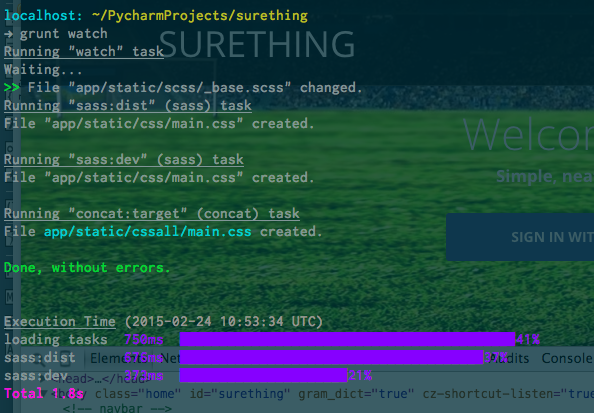
\includegraphics[width=.60\linewidth]{impl/images/gruntInAction}
		\caption{A screenshot from the terminal output running Grunt.} \label{fig:using:gruntinaction}
	\end{center}
\end{figure}
	
In addition, RequireJS  \cite{documentation:RequireJS}, a powerful asynchronous script loader will be used for effective management of JavaScript dependencies. It can load modules in asynchronous manner if desired and thus improve overall website performance.

\subsection{Back End}
\label{subsec:backend}
For making reasonably accurate football results predictions the application requires latest footaball data. Live data would have to be frequently loaded into the system and processed in an appropriate way. Therefore, there would be a need for at least one separate module dealing with a third party football data API and containing business logic to manipulate the received data. The API wrapper is expected to be integrated into the web application, but separated from the presentation, it also has to be relatively easy to execute as a standalone module, encouraging a nicely decoupled design. Based on the above assumptions, Python was chosen as a primary back end language for this project being known as a language well suited to data manipulation.

The back end of the web application will be built using Python web framework Flask \cite{documentation:Flask}. It is a lightweight framework (the official name is "Python microframework") with a great choice of third-party libraries (e.g. Flask-SQLAlchemy or Flask-Login) that can extend the feature set of the framework core in various ways. Flask application is minimalist to begin with, but it can grow with the project needs. For the purpose of this project this is an advantage compared to the full-featured frameworks like Django that have a lot of functionality already built-in in the basic installation. In addition, availability of developer-friendly documentation and low learning curve makes Flask a short way to get a simple, Python-powered web site up and running. Therefore, Flask appears to be a great choice for a small project like SureThing. 

SQLAlchemy was chosen as database solution for this project \cite{documentation:SqlAlchemy}. This is a powerful database framework that supports several databases back ends and offers the high-level Object Relational Mapper (for short, ORM). Using ORM provides a great level of abstraction when working with databases. For example, SQLAlchemy uses classes that map to each table in a database. This means that the records interaction can be kept the same regardless of the underlying database system. This offers a lot of flexibility and, for example, allows to use different database systems for development and production environment. According to \cite{book:Grindberg2014FlaskWebDevelopment}, "Flask-Migrate extension, based on a migration framework Alembic and written by a lead developer of SQLAlchemy, provides a powerful solution to handle database alterations and make database schema updates easily manageable" 

\section{Application Architecture}
\label{sec:applicationarchitecture}
Application architecture is a base of a good quality software. The architecture of SureThing was from a big part dictated by the used framework Flask, that uses a variation of MVC for Python called "MTV" (Model-Template-Controller). Nando Florestan \cite{article:goodArchitecture} in his blog post describes this pattern in the following way:

\begin{quote}
"The template contains HTML content and presentation logic. It is written in a templating language ... It gets data from the view and outputs a web page. The view (also sometimes called “controller”), written in Python, is just glue code. It uses the web framework to put everything together. The model layer is essentially a persistence layer: its most important dependency is SQLAlchemy. The model knows how to save the data, constituting the most reusable code in the entire project."
\end{quote}

However, on the top of the standard MVC architecture SureThing requires few extra components to manage the loading of the data from an external source. Hence, this is the final layout of the application architecture:

\begin{itemize}
    \item \textbf{Model Layer.} Contains Python classes that represent database models and related logic. According to Florestan \cite{article:goodArchitecture}, model layer "represents the essence of your system without the details of a user interface."
    \item \textbf{View Layer.} Holds association between URL rules and view functions that are defined with a help of a module-level decorator \emph{route()}. Below can be found an excerpt from the application code, a header of a view function that represents the dashboard page. When a browser requests \url{/dashboard} URL, the associated view function is called and the return value is sent back to the browser. 

\begin{figure}[H]
    \begin{center}
        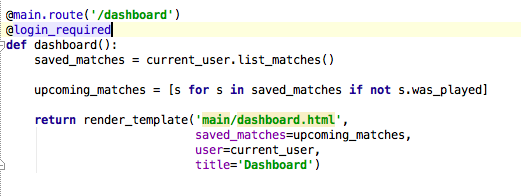
\includegraphics[width=.70\linewidth]{impl/images/routeExample}
        \caption{Dashboard view function.} \label{fig:using:routeexample}
    \end{center}
\end{figure}     
        
    \item \textbf{Template Layer.} This is the mediator layer between an HTTP request and the application logic. It consists of a number of Jinja2 templates holding only     presentation logic. 
    \item \textbf{External Services Layer} \cite{article:goodArchitecture}. Contains API wrapper class that accesses and manipulates live football data. In general, the functionality of the application can be further extended in many ways. In the future, Football-API might not be the only external source of data. The project might make use of another third-party API or even use web scraping technique to extract data from other websites . Eventually, all additional modules related to the interaction with external sources of data will become part of this layer.
    \item \textbf{Threading.} The application requests live football data frequently. Loading the data is a costly I/O operation that may become a bottleneck unless performed asynchronously. Threading component of the apllication defines a class \emph{DataUpdateThread} that takes care of writing the data to the server every 100 seconds. This task is performed in a separate thread. 
\end{itemize}

During the development process, a lot of effort was put into keeping the Template Layer as thin as possible in order to reduce the loading time in the browser and improve the overall performance of the application.

\section{Patterns And Conventions}
\label{sec:patternsandconventions}
Flask offers an excellent extendable core of functionality; its API is also very minimalistic and easy to understand. One of the  main advantages of this framework is that it gives developer a lot of freedom to decide how to structure the application. As Matt Wright \cite{article:howIstructureMyFlaskApps} puts it: " without patterns or conventions your applications will loose architectural integrity and be difficult to understand by others". In this section a number of various patterns, conventions and tools used during the implementation phase will be described and explained. 

\subsection{Application Factory}
\label{subsec:applicationfactory}
The use of factory pattern is crucial to a Flask application. For example, SureThing app defines various configurations to be used in different environments (development, testing, production). However, because the application instance is created in the global scope, there is no way to apply those configurations. The problem is that "by the time the script is running, the application instance has already been created, so it is already too late to make configuration changes." \cite{book:Grindberg2014FlaskWebDevelopment} To get around this problem a creation of the application was moved into a separate function, \emph{create\_app()}. The name of configuration name is passed into the function as a parameter. This solution also allows us to create multiple instances of the application and make testing of various confurations easier.\cite{documentation:FlaskApplicationFactories} 

\begin{figure}[H]
	\begin{center}
		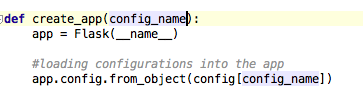
\includegraphics[width=.50\columnwidth]{impl/images/createApp}
		\caption{Function responsible for creating the application instance.} \label{fig:using:createapp}
	\end{center}
\end{figure}

\subsection{Blueprints}
\label{subsec:blueprints}
Blueprints are related to the View Layer introduced in the section Application Architecture \cite{sec:applicationarchitecture}. A large application is divided into smaller parts and each part is implemented with help of a blueprint. This concept helps to develop a \emph{modular} web application. SureThing was divided into two parts: \emph{main} and \emph{auth}. \emph{auth} holds the endpoints associated with the authentication and user profile related tasks, for example \emph{login()}, \emph{edit\_profile()}. On the other hand \emph{main} is in charge of the rest of the application. Notice how those different blueprints are registered on the application instance inside the \emph{create\_app()} function:

\begin{figure}[H]
	\begin{center}
		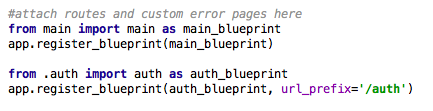
\includegraphics[width=.50\columnwidth]{impl/images/blueprintsRegistration}
		\caption{Blueprints registration.} \label{fig:using:blueprintsregistration}
	\end{center}
\end{figure}

\subsection{Database Migrations}
\label{subsec:databasemigrations}
The database scheme for this project was designed in an iterative way, models and relationships between them were added gradually as the application was growing. Therefore, it was crucial to find a tool that allows effortless updates of the database. To manage frequent database updates was used Alembic database migration tool that was developed specifically by Mike Bayer, the author of SQLAlchemy. The tool can be added to Flask as an external plugin, Flask-migrate. After installation and initial configuration of the plugin, it allows to migrate the database with two simple commands to be subsequentially run in the terminal: \emph{db upgrade} and \emph{db migrate}. Alembic makes migration easier and prevents the developer from the necessity to delete and recreate the database each time there is a need for migration.

\subsection{Exceptions}
\label{subsec:exceptions}
In general, it is considered a good practice to take advantage of standard libararies of a programming language, in our case Python. First of all, it allows developer to save time implementing a piece of functionality from scratch. Secondly, it makes it easier for other developers to read and maintain the code. Exceptions are built into Python at the language level. Using them will lead to cleaner code and will not have any impact on the performance. "In a way, try blocks are like transactions. [The] catch has to leave ... program in a consistent state, no matter what happens in the try. For this reason it is good practice to start with a try- catch- finally statement when you are writing code that could throw exceptions " \cite{book:martin2011robert}.
 
SureThing will make use of Exceptions in order to identify and manage failures when making an API call over HTTP. The FootballAPIWrapper class has a private method that calls the API and collects the data in a JSON format from the remote server: \emph{\_call\_api(action=None, **kwargs)}. The method takes into account the possibility of errors occuring during code execution. When the program calls the API, either JSON data is returned or an Exception is thrown. 

As it can be seen from the method definition above, one of the required parameters is \emph{action} that is set to None, unless the value is passed in during the method call. Action is a string that needs to be added to the base url in order to indicate the set of data that is being accessed. Specifying the action is required by the API and the possible values of the parameters (actions) are: competition, standings, today, fixtures, commentaries. For example action \emph{today} will returns the matches scheduled today. The \emph{\_all\_api} method will raise an Exception, if the action is not being supplied. Various exceptions are thrown when the program is attempting to connect to the remote server \cite{article:httpRequestsExceptions}. Python library \emph{requests} is used to take care of this type of errors \cite{documentation:PythonRequests}. If the domain name does not resolve, the HTTP request will fail before we establish connection. In that case, the program will throw a \emph{requests.exceptions.ConnectionError}. If the remote server is not functioning or the request is structured incorrectly, the server will respond with an bad response status code and the \emph{\_call\_api} method will raise a \emph{requests.exceptions.HTTPError}.

\section{Other Implementation Processes}
\label{sec:otherprocesses}
In this section a number of other implementation processes and used tools will be discussed.

\subsection{PEP8}
\subsection{PyLint}

\subsection{Version Control}
\label{subsec:git}
Git version control system was used throughout the development process. Git is known for being a very useful tool for collaboration across teams of developers. However, it has also many benefits for a solo developer. For example, it helps to track changes and restore previous versions of a project, as well as view the code at any point in the past. The project codebase was uploaded to GitHub that is \cite{wiki:GitHub} "a web-based Git repository hosting service, which offers all of the distributed revision control and source code management (SCM) functionality of Git as well as adding its own features... [It also] provides web-based graphical interface". For this project GitHub issue tracker was used as a "to-do list" to keep the record of tasks ("issues" in GitHub terminology) that needed to be completed in each agile iteration. Custom labels were used to distinguish different types of issues in the GitHub issue tracker, for example, "performance", "design", "bug", "optional", etc. 

\begin{figure}[H]
	\begin{center}
		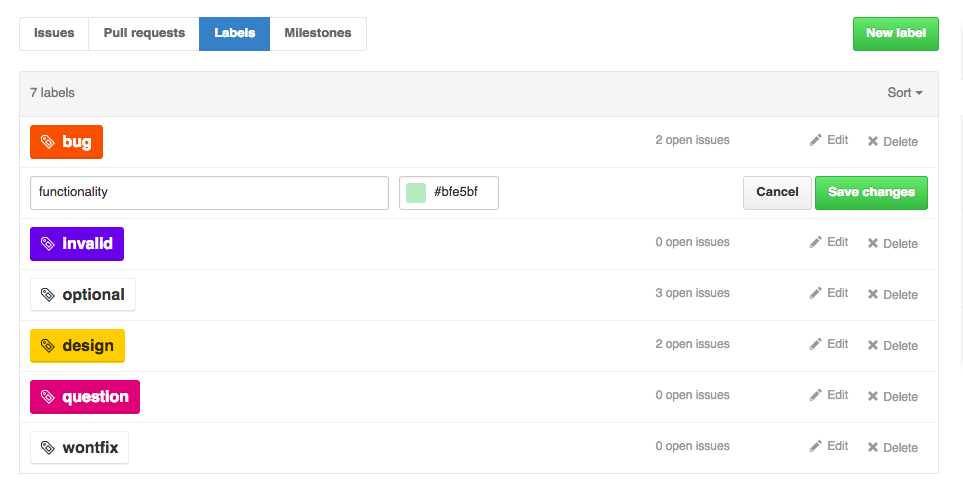
\includegraphics[width=.90\columnwidth]{impl/images/githubLabelsChoice}
		\caption{GitHub allows developers to add custom labels.} \label{fig:using:githublabelschoice}
	\end{center}
\end{figure}

GitHub also allows the users to filter out the issues of a similar type, based on the assigned label.

\begin{figure}[H]
	\begin{center}
		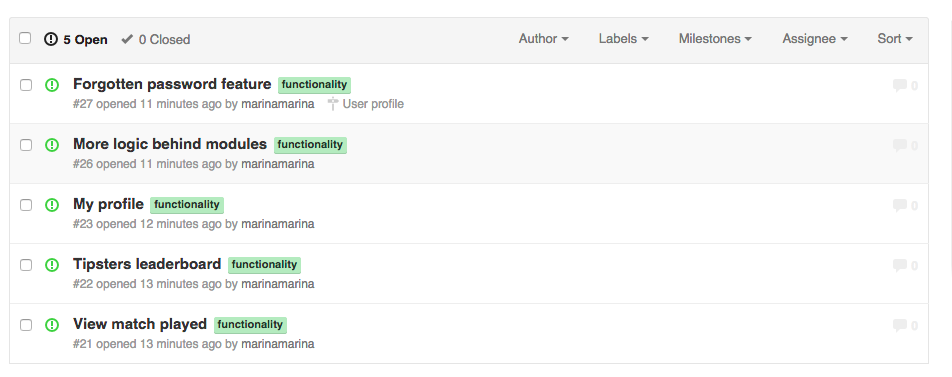
\includegraphics[width=.90\columnwidth]{impl/images/githubFunctionalityIssues}
		\caption{GitHub. Issues related to the functionality of the application.} \label{fig:using:githubfunctionalityissues}
	\end{center}
\end{figure}

Critically speaking, I missed the option to assign issues various level of importance and order the issues based on their priority.

\subsection{Own Validation in Forms}
\label{subsec:validations}
Flask-WTF is a Flask extension that offers integration with WTForms and it was used to handle forms in this project. In order to make sure the application is secure, the validation has to be implemented preferably on the server side or both on the client- and server-side of the application. WTForms has many built-in validators that can simplify developer's life. For example \textbf{DataRequired} makes the input field mandatory, \textbf{Email} checks that the provided input is a valid email address, \textbf{EqualTo} helps to ensure that the passwords in the fields "Password" and "Confirm Password" supplied during the user registration are identical. However, sometimes the built-in functionality does not cover all the application needs. In that case, there is an option to create a custom validator that is a basically a Python function returning another function (a validator) that throws an exception every time the user violates the prescribed validation rule. Custom validators can be imported into the module describing forms and used in the same way as a built-in validator would be used. I have separated the validators out into a separate module. The set of custom validators can be further extended, however, there is just one at the moment: \emph{validator\_user\_already\_registered()}. 

\begin{figure}[H]
	\begin{center}
		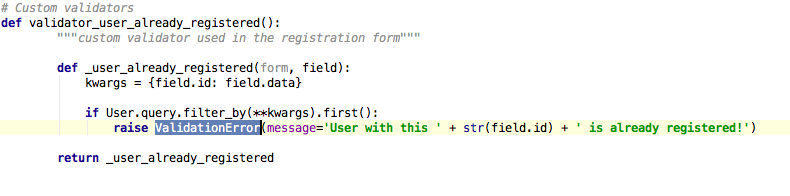
\includegraphics[width=.90\columnwidth]{impl/images/customValidator}
		\caption{Validator function that checks if user with this username has already been registered with the SureThing application} \label{fig:using:customValidator}
	\end{center}
\end{figure}

In the example above the validator function checks if a user with provided username is already in the database. If the user is found, the ValidationError exception is thrown and the new user is prevented from submitting the form.

\subsection{Custom Macros}
Jinja2 is a default template engine that comes in one package with Flask. It is also one of the most widely used template engines for Python. In order to add some extra presentation logic to our application, custom macros can be used. Jinja2 macro is simply a template function that can be used within HTML in order to avoid developers writing repetitive code. For this project I found macros extremely useful. Custom macros were separated out into a separate template file \emph{\_macros.html}.

One of the example usages was rendering form fields. Each form field related macro contained a piece of HTML code specifically designed for forms in this application, as well as logic for dispaying error messages. Among this type of macros can be named \emph{render\_field(field)}, \emph{render\_checkbox(field)}, \emph{render\_submit\_field(field)}. Some of those macros needed to be adjusted to enable their usage in a specific view. These are the examples of such "adjusted" macros: \emph{render\_submit\_field\_match\_preview(field)}, \emph{render\_embedded\_field(field)}. For example, \emph{render\_field} takes care of rendering any standard input field accross the application, whereas \emph{render\_embedded\_field(field)} manages rendering an input field embedded within a prediction module on the Upcoming Match View. 

Another macro, \emph{teamkitimage(match, home=1)} renders an image representing a football club. Based on the provided arguments, the function displays an image of a home or away team kit for a specific club. 

\subsection{Integration with third-party API}
Many production Python web applications rely on external application programming interfaces (APIs). API can be also reffered to as "third party services" or "external platform" \cite{article:API_Integration}.  SureThing requires constant access to current football data. After choosing an appropriate API, it has to be integrated into the application. 

There is a variety of tools available for developers for accessing web APIs. Those three options were considered when choosing an appropriate tool:
	
\begin{itemize}
	\item Helper library (such as Runscope or Apiary)
	Using a helper library has an overhead of learning how to use another piece of software.
	\item urllib2, standard Python module
	\emph{urllib2} module offers very simple implementation and provides most of the required HTTP capabilities, but the API is thoroughly broken and features critical for performance are missing, for example connection re-using/pooling. 
	\item urllib3
	\item requests, another Python library for handling HTTP requests. It offers a lot of control over the HTTP calls through the use of its powerful features.
\end{itemize}
		
After some experiments with other urllib2, urllib3 and requests, \emph{requests} was chosen as the libarary for this project.
		
All interaction with the Football-API, including processing the received data, was separated out into a module \emph{football\_api\_wrapper.py} or just "wrapper" for short. This module contains only one class, FootballAPIWrapper. Fields of the class accomodate the key elements of the interaction with the API that will be re-used in different methods of the wrapper, for example base url, path to the data directory.
	
\begin{figure}[H]
	\begin{center}
		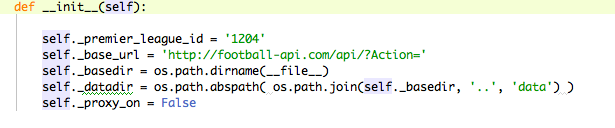
\includegraphics[width=.90\columnwidth]{impl/images/footballApiWrapperFields}
		\caption{Football API wrapper, fields} \label{fig:using:footballapiwrapperfields}
	\end{center}
\end{figure}
	
To get the response from Football-API takes about 11s, therefore it is nessessary to move the API calls into a task queue so they do not block the HTTP request-response cycle for the rest of the web application.

\subsection{Visual Effects}
A number of visual effects was implemented with the help of jQuery, AJAX and the Websockets (Flask extention Flask-SocketsIO) to improve the user experience. 

\subsubsection*{Alerts}
A good example is an alert dismissal. SureThing generates many alerts that give the user feedback with regards to the action they have just taken. User has to dismiss the alert manually each time. To avoid this extra thing for a user to do, the alerts are removed from the page using jQuery fadeOut() and then slideUp() animation methods that fades the pop-up and then removes it with a sliding motion after 200ms of its appearance on the page. For compactness the screenshot shows the page opened in a browser simulation of an iPhone screen size. Responsive web design with regards to this project will be examined in more detail in the following subsection.

\begin{figure}[H]
	\begin{center}
		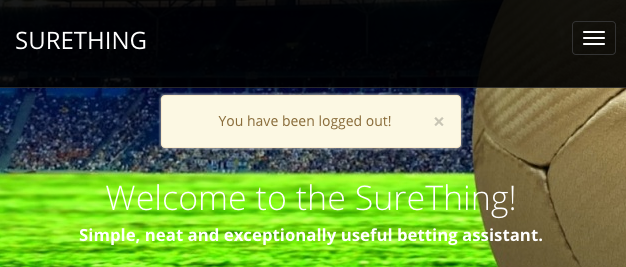
\includegraphics[width=.60\columnwidth]{impl/images/alert}
		\caption{An example of an alert on the page appearing after user has logged out} \label{fig:alert}
	\end{center}
\end{figure}

\begin{figure}[H]
	\begin{center}
		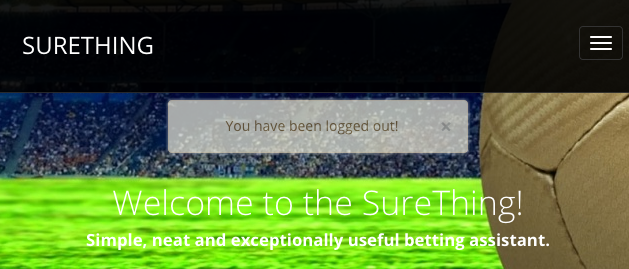
\includegraphics[width=.60\columnwidth]{impl/images/alertFadeOut}
		\caption{The same alert fading out.} \label{fig:alertFadeOut}
	\end{center}
\end{figure}

\subsubsection*{New message notifications}
Another example is a new message notification. Once user received a new in-app message notifying them about the results of their bets, the envelope-shaped icon on the top navigation menu that represents the in-app Inbox turns orange. 

\begin{figure}[H]
	\begin{center}
		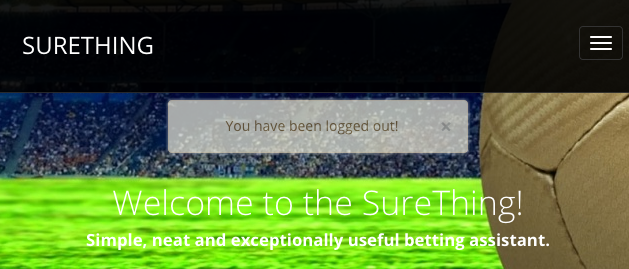
\includegraphics[width=.60\columnwidth]{impl/images/alertFadeOut}
		\caption{The same alert fading out.} \label{fig:alertFadeOut}
	\end{center}
\end{figure}

When user navigates to the Inbox and reads or deletes all the new messages, the icon immediately turns greyindicating that there are no more unread messages in the box.
 
\begin{figure}[H]
	\begin{center}
		
\includegraphics[width=.60\columnwidth]{impl/images/newMessagesDesktopView}
		\caption{You have new messages. Desktop View.} \label{fig:newmessagesdesktopview}
	\end{center}
\end{figure}

This is what the same top navigation menu looks like for mobile users. 

\begin{figure}[H]
	\begin{center}
		
\includegraphics[width=.60\columnwidth]{impl/images/newMessagesMobileView}
		\caption{You have new messages. Mobile View.} \label{fig:newmessagesmobileview}
	\end{center}
\end{figure}

User has opened the last unread message and the message icon has turned grey. Notice, how the top navigation menu partly covers the message view. The menu rolls back into a compact mode once the user clicks on the menu icon in the top right corner.

\begin{figure}[H]
	\begin{center}
		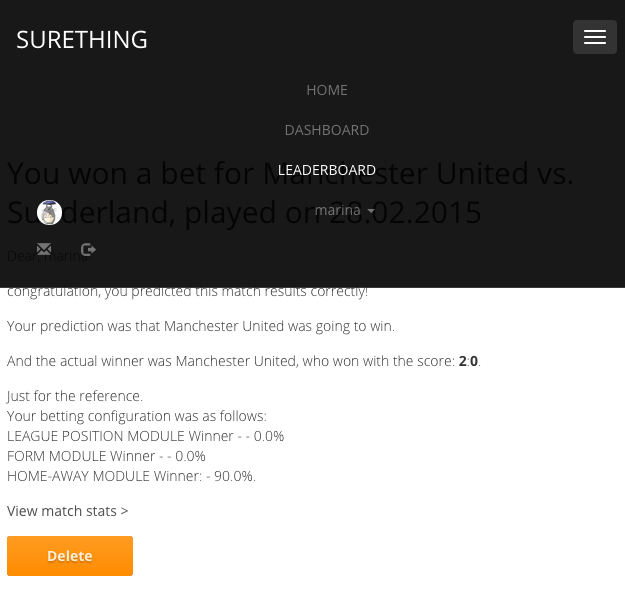
\includegraphics[width=.60\columnwidth]{impl/images/noMoreNewMessages}
		\caption{User just read the last new message, the icon turns grey.} \label{fig:nomorenewmessages}
	\end{center}
\end{figure}

\subsection{Responsive Design}
According to the popular portal Statista, "As of 2013, worldwide mobile phone internet user penetration was 73.4 percent. In 2017, figures suggest that more than 90 percent of internet users will access online content through their phones" \cite{statistaReport}. There is no doubt that developers need to adapt to the increasing combinations of screen resolution and browsers used by people to access information online. The solution to the expanding variability of the web is to develop a layout that can adapt to any viewport. This approach is known as \emph{responsive web design}. The term was first used by Ethan Marcotte. He combined three already known techniques (flexible grid layout, flexible images, and media and media queries) into a unified approach \cite{book:frain2012responsive}. 

Based on the above, we should assume that the majority of users will access our website through a device that is not a desktop. We need a good fluid grid to build a responsive web application. To handle the responsiveness and to increase development speed SureThing utilises Bootstrap framework \cite{documentation:Bootstrap3}. that offers an responsive fluid grid system that can adjust to the variety of devices or screen sizes. The framework has also predefined classes that can be used to change the page layout options, for example to specify how many columns in the grid system an element will occupy or to set the breakpoints at which the columns stacked on small devices will become horizontal on medium/large devices. 

SureThing is a fully responsive web application, and the minimum screen resolution supported is 640 x 960 pixels (an example device is iPhone 4). These are the screenshots of some of the application pages tested with this resolution:

\begin{figure}[H]
	\begin{center}
		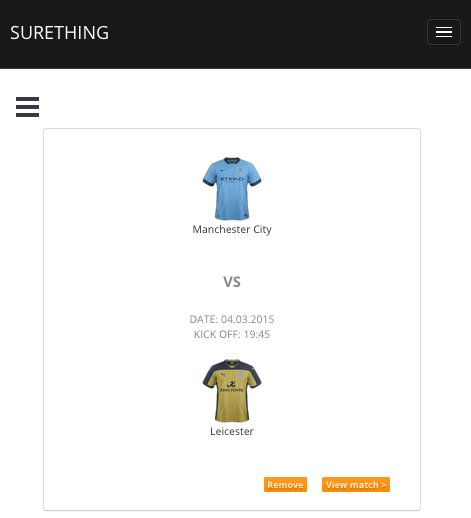
\includegraphics[width=.50\columnwidth]{impl/images/responsiveDashboard}
		\caption{Dashboard view, DVGA screen size.} \label{fig:using:responsivedashboard}
	\end{center}
\end{figure}

\begin{figure}[H]
	\begin{center}
		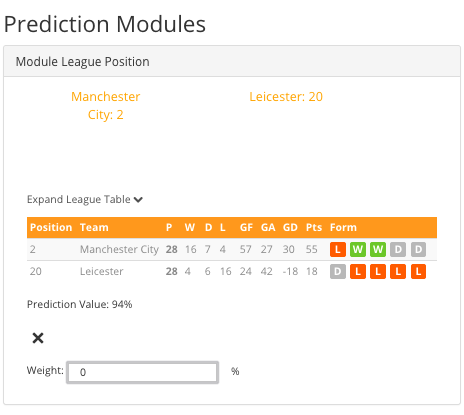
\includegraphics[width=.50\columnwidth]{impl/images/responsiveModuleLeaguePosition}
		\caption{Module League Position in the Upcoming Match View, DVGA screen size.} \label{fig:using:responsivemoduleleagueposition}
	\end{center}
\end{figure}

\section{Features Implementation}
In this section will be described the technical details of the project implementation. Each susbsection is bound to the high level feature of the application, as indroduced in the chapter "Requirements Analysis" \ref{sec:functionalrequirements}. "User journey", or possible user interactions with the system, will be demonstrated for each view.

\subsection{Authentication and User Profile}

\subsubsection*{Authentication}
The application requires authentication functionality. In order to simplify the development process, a useful Flask extention, Flask-Login, was utilised to handle the common tasks of logging in and out, as well as new users registration. For the new users the application offers a registration form. On form submission, SureThing sends user an email with verification token, expecting them to confirm the email address and complete the registration. It should be noted that both username and email address provided during the registration should be unique, otherwise the application throws a validation error.

\begin{figure}[H]
	\begin{center}
		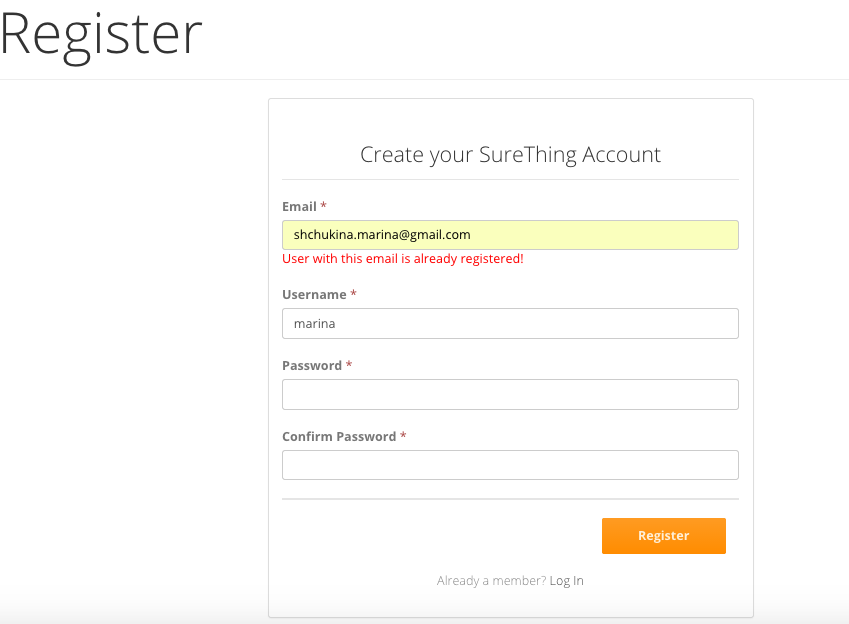
\includegraphics[width=.90\columnwidth]{impl/images/registrationFormError}
		\caption{SureThing offers registration form for the new users. However, the email address is expected to be unique.} \label{fig:registrationformerror}
	\end{center}
\end{figure}

Once user has created a SureThing account, they can login using a standard login form.  An email address and a password are both required fields. A validation error will be thrown in case the provided email or password are invalid, or the user with the provided email address was not found in the database.

An authorised user will see the icon with their avatar picture in the top right corner of the application navigation menu, as it can be seen in the screenshot below. Gravatar stands for "Globally recognized avatar" and it is one of the most popular avatar services. User can register with the service (\url{http://gravatar.com}) and upload their images that can be used as avatars accross many popular websites, such as GitHub (\url{http://www.github.com}), Stackoverflow (\url{http://www.stackoverflow.com}) and WorldPress (\url{http://www.worldpress.com}). Therefore, newly registered user does not have to upload an avatar image to be used in our application. The app will access the avatar associated with their email address and pull it from the Gravatar servers. 

\begin{figure}[H]
	\begin{center}
		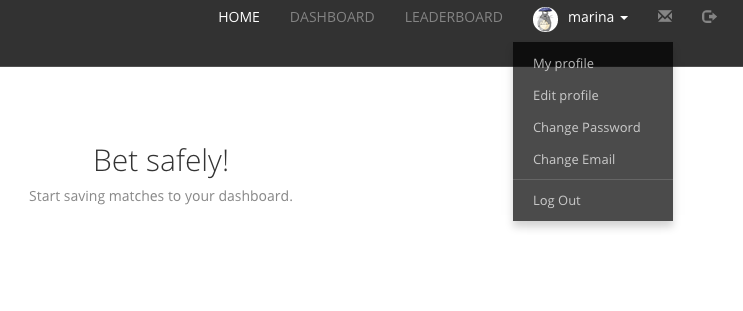
\includegraphics[width=.90\columnwidth]{impl/images/gravatar}
		\caption{User settings and the profile page can be accessed by clicking on the gravatar icon located on the application navigation menu panel.} \label{fig:gravatar}
	\end{center}
\end{figure}

In case the user is not registered with the Gravatar, SureThing will generate a dummy avatar to be used in the application.

\begin{figure}[H]
	\begin{center}
		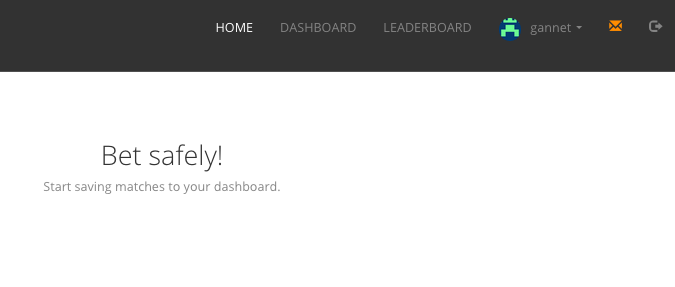
\includegraphics[width=.90\columnwidth]{impl/images/dummyGravatar}
		\caption{An example of a dummy gravatar for user \textbf{gannet}.} \label{fig:dummygravatar}
	\end{center}
\end{figure}

\subsubsection*{User Profile}
The options available in the dropdown menu, as displayed in the figure ~\ref{fig:gravatar}, enable the users editing their profiles, changing password and email address. 

\begin{figure}[H]
	\begin{center}
		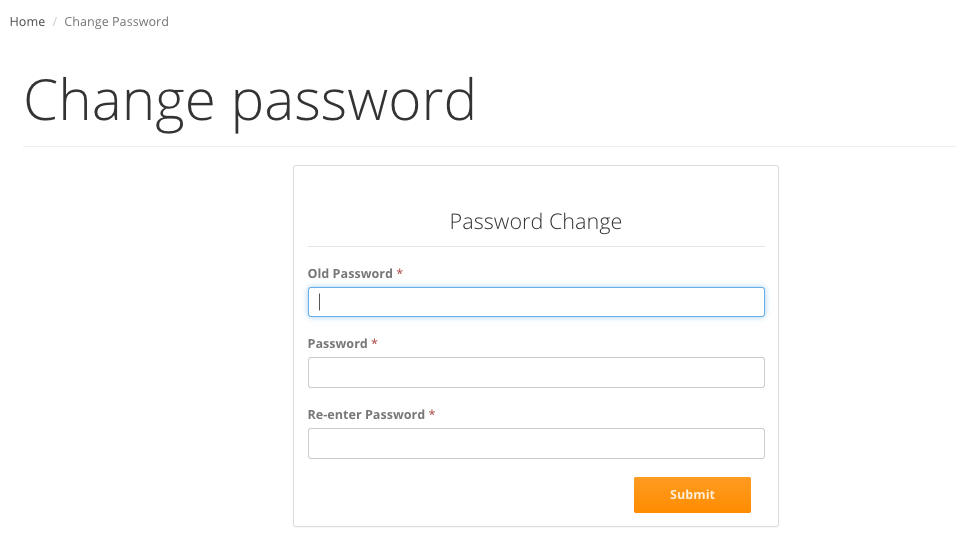
\includegraphics[width=.90\columnwidth]{impl/images/changePassword}
		\caption{Users can change their passwords for securiy reasons.} \label{fig:changePassword}
	\end{center}
\end{figure}

\begin{figure}[H]
	\begin{center}
		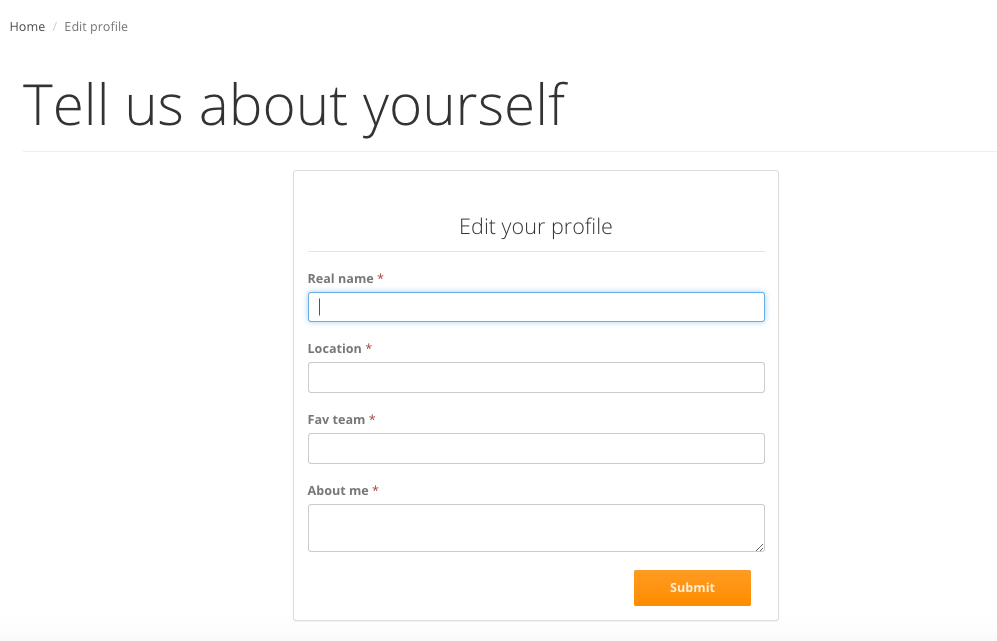
\includegraphics[width=.90\columnwidth]{impl/images/editProfile}
		\caption{After the registration users can share more information about themselves by editing their profile.} \label{fig:editprofile}
	\end{center}
\end{figure}

Clicking on the dropdown option "Profile" will take the user to a separate page containing all the information about the user, for example: profile information, preferences, section "about me", recent won bets including the prediction weights used for these bets, etc. 

\begin{figure}[H]
	\begin{center}
		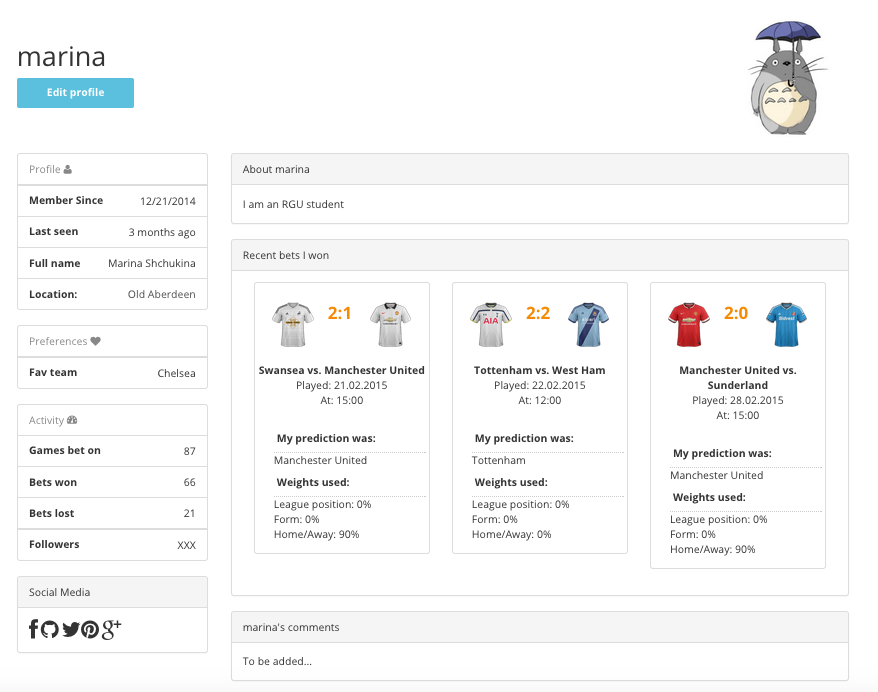
\includegraphics[width=.90\textwidth]{impl/images/profile}
		\caption{User profile page.} 
		\label{fig:profile}
	\end{center}
\end{figure}

\subsubsection*{User Journey}
\label{subsec:authandprofileuserjourney}
User can also navigate to the "Edit profile" form in a different way, namely by clicking on the light blue "Edit Profile" button located in the top left corner of the profile page. 

\subsection{Matches Overview}
Matches Overview is a view displayed on the main page of the application. It contains lists of upcoming and played matches and the user can toggle between those two lists using navigation buttons. In both lists matches are grouped by dates as follows:

\begin{figure}[H]
	\begin{center}
		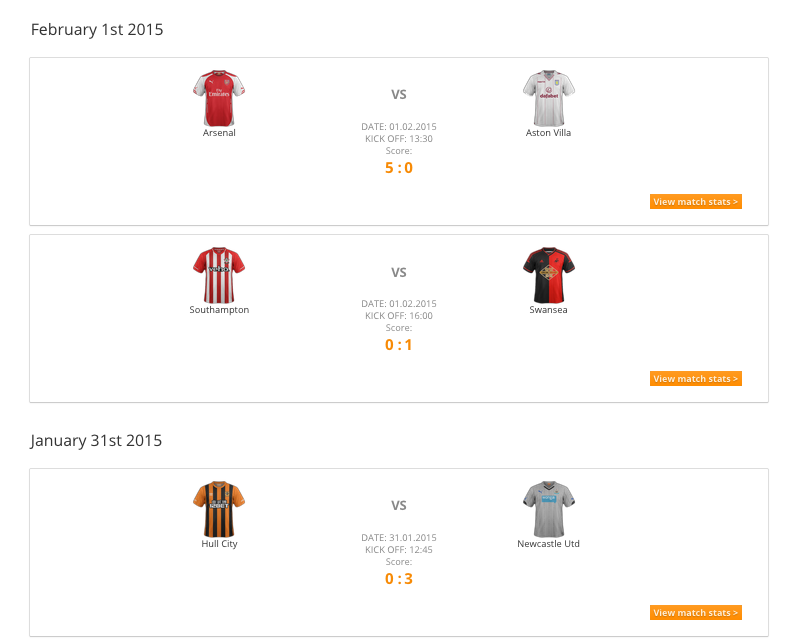
\includegraphics[width=.90\textwidth]{impl/images/matchesGrouped}
		\caption{Matches in the overview are grouped by dates sorted in ascending order.} \label{fig:using:matchesgrouped}
	\end{center}
\end{figure}
 
Each panel representing a match contains the most basic information about the event, such as names of participating teams, kick-off date and time. The screenshot below is an example of a panel displaying an unplayed match. The navigation buttons can be seen just above the first match in the list. Match already saved to the Dashboard by the authenticated user is indicated by a floppy disk icon on the right hand side of the panel.

\begin{figure}[H]
	\begin{center}
		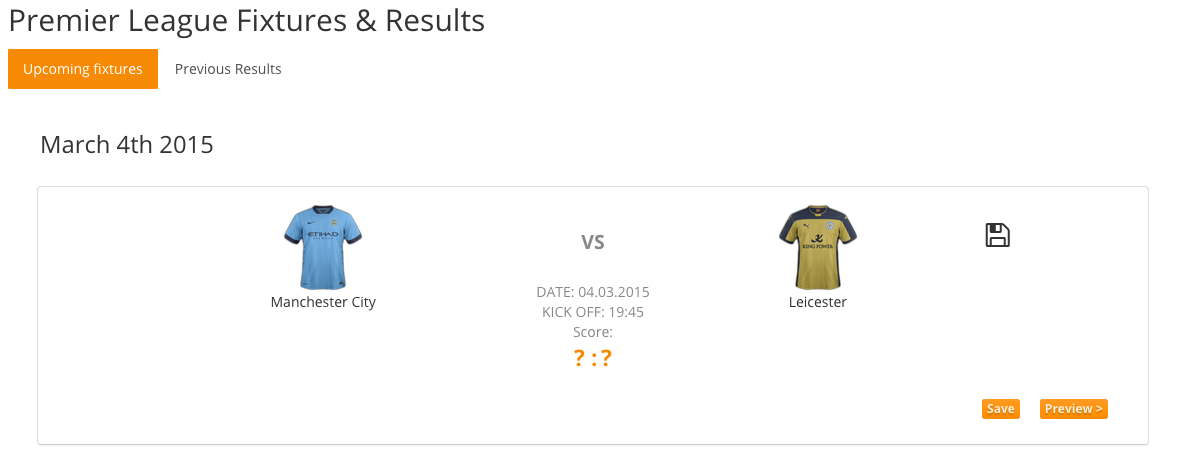
\includegraphics[width=.90\textwidth]{impl/images/unplayedMatch}
		\caption{Example of an unplayed match displayed in the overview.} \label{fig:using:unplayedmatch}
	\end{center}
\end{figure}

Below can be found a screenshot of a played match panel. Notice that the final score of the match is displayed and instead of two buttons "Save" and "Preview" there is only one button - "View match stats".

\begin{figure}[H]
	\begin{center}
		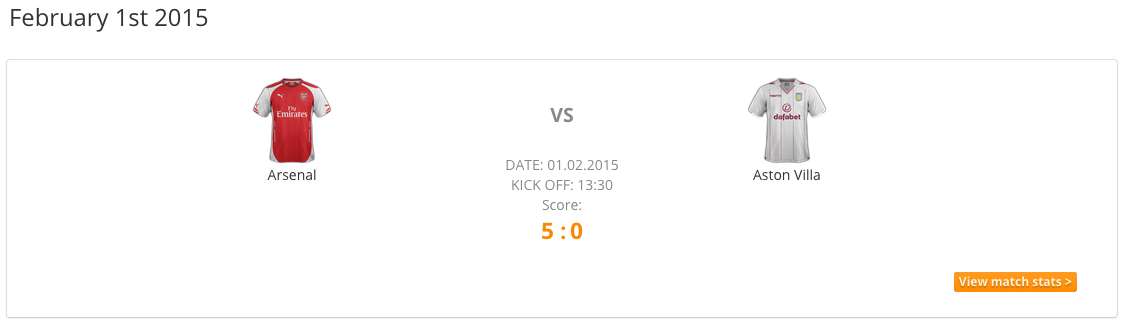
\includegraphics[width=.90\textwidth]{impl/images/playedMatch}
		\caption{Example of a played match displayed in the overview.} \label{fig:using:playedmatch}
	\end{center}
\end{figure}

In case the match is being played at the very moment, it still belongs to the list of "unplayed" matches and is displayed with a small badge "LIVE", indicating live event. A match is considered as "played" as soon as the full time score is available. Hence, it is possible to make "bets" until the moment the match is considered "played".

\begin{figure}[H]
	\begin{center}
		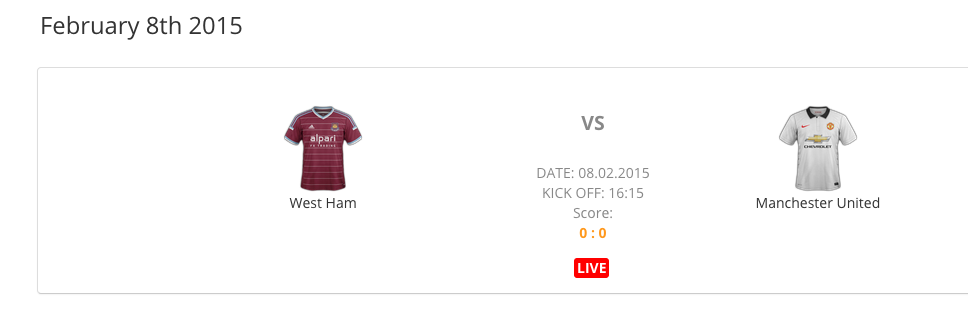
\includegraphics[width=.90\textwidth]{impl/images/liveMatch}
		\caption{Example of a live match displayed in the overview.} \label{fig:using:livematch}
	\end{center}
\end{figure}

\subsubsection*{User Journey}
\label{subsec:matchesoviewuserjourney}
Just above the list can be found simple navigation allowing to switch between the lists of unplayed and played matches. On the right hand side of each list item there is a "Preview" button for an upcoming match and a "View match stats" button for a played match. By clicking those buttons user can navigate to views with more detailed information about the match (\emph{Upcoming Match View} or \emph{Played Match View}). User can save the match to the dashboard by clicking "Save" button. This action can be carried out only for an unplayed match.  

\subsection{Upcoming Match View}
\label{subsec:implementupcomingmatchview}
Implementation of this view was one the most complex development tasks of the whole project. This is the essense of SureThing - view allowing the user to predict match results. 

Authenticated SureThing user can navigate to this view either by clicking a "Preview" button on an upcoming match panel in the \emph{Matches Overview} or by clicking the same button on a saved match panel in the user \emph{Dashboard} (if the match has already been saved by the user). Depending on the user route to this view, the Upcoming Match Preview will be displayed differently.

\subsubsection*{Read-only mode}
If the user is coming to the Upcoming Match Preview from the \emph{main page}, the view will display the match header (containing general information about the teams, last played game, match kick-off time and date, etc.) and a list of prediction modules with \textbf{prediction values} calculated based on the relevant piece of statistics for each of the teams. These are the prediction modules available in this view: 

\begin{enumerate}
	\item Module League Position
	\item Module Form
	\item Module Home/Away
\end{enumerate}

"Save" button can be found at the very bottom of the view.

\begin{figure}[H]
	\begin{center}
		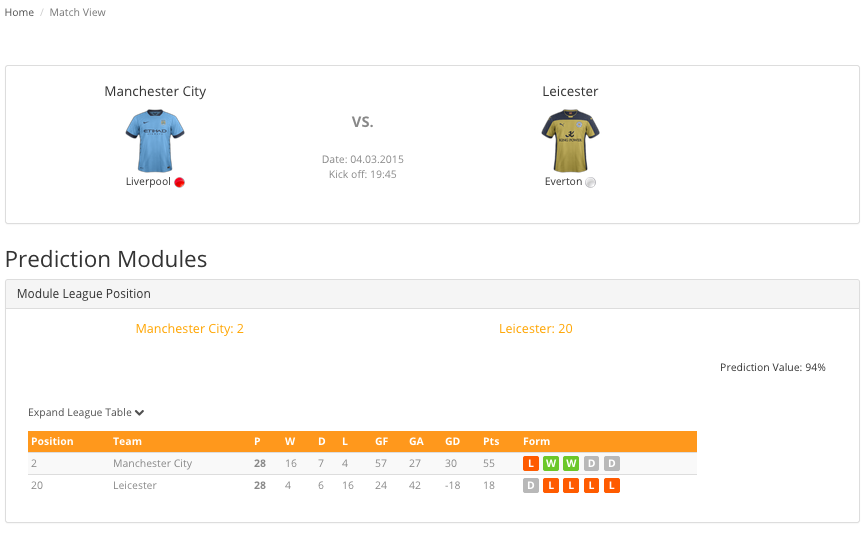
\includegraphics[width=.90\textwidth]{impl/images/upcomingMatchView}
		\caption{Upcoming Match View in the "read-only" mode: match header and the first prediction module, Module League Position.} 
		\label{fig:using:upcominmatchview}
	\end{center}
\end{figure}

This information should be sufficient for the user to decide, whether it is worth saving the match to the dashboard for a later revision. An unauthorised user would be able to see the same content, but the "Save" button will be disabled. We can say that if user navigates to the Upcoming Match View from the main page, they can see the view in the \textbf{read-only mode}. It is also important to note that this is one of few views that are available for an unauthorised user.

\subsubsection*{Prediction mode}
In case user has already saved the match to the dashboard and navigates to the view by clicking on a saved match panel, the view will enable the prediction feature. This time the view is displayed in the \textbf{prediction mode}. In each of the prediction modules user will be able to see an embedded input field with weight percentages inside the field. Below can be found a screenshot of a same part of the view as the one above, displayed in prediction mode.

\begin{figure}[H]
	\begin{center}
		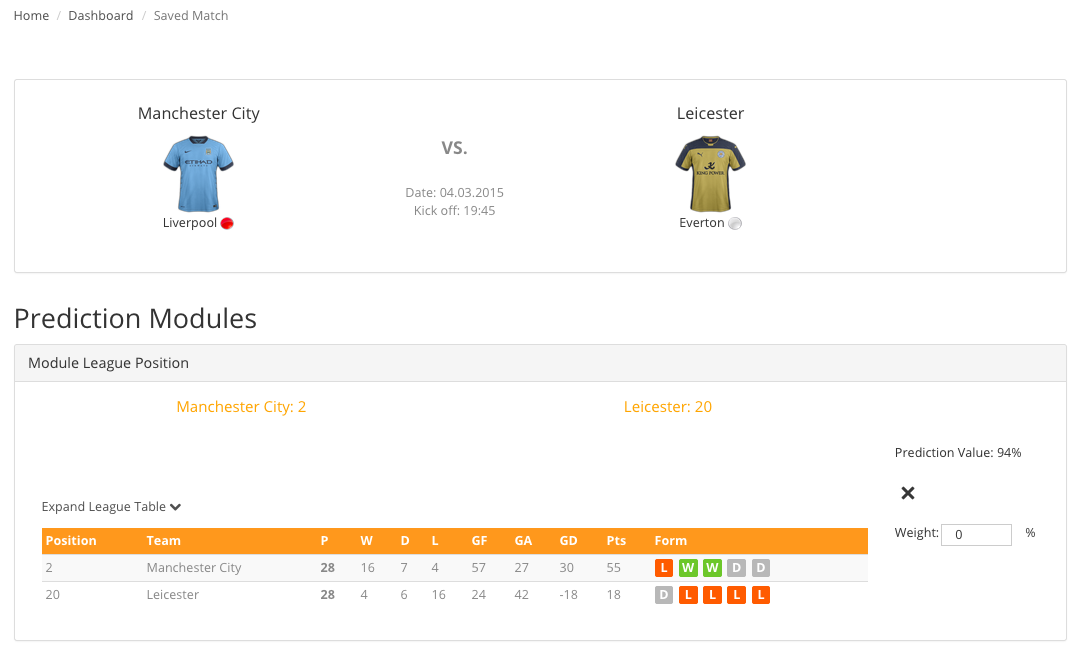
\includegraphics[width=.90\textwidth]{impl/images/upcomingMatchViewSM}
		\caption{Upcoming Match View in the "prediction" mode: match header and the first prediction module, Module League Position.} 	  \label{fig:using:upcominmatchviewSM}
	\end{center}
\end{figure}

The values displayed inside the fields will be used for calculating the overall match result prediction. If this is the first time user previews the match, the prediction weights will be either the \textbf{system default} (in case user has not set the prediction settings in the dashboard yet) or the \textbf{user default} prediction settings. If user has already visited this page before and set the match specific settings, the values displayed inside the input fields will be the \textbf{match specific} ones. Any module can be eliminated from the prediction by setting its weight to 0\%. The total sum of prediction weights must equal to 100\%.

These are the prediction modules available to the user in the prediction mode:

\begin{enumerate}
	\item Module League Position
	\item Module Form
	\item Module Home/Away
	\item User Hunch
\end{enumerate}

Notice, the extra module is available in this view - User Hunch. This module is very important to the prediction process. User can personalise the prediction by choosing Home, Away or Draw value in the User Hunch module panel. The module will be explained in more detail in the subsection, "Prediction" \cite{subsec:predictionimplementation}

\begin{figure}[H]
	\begin{center}
		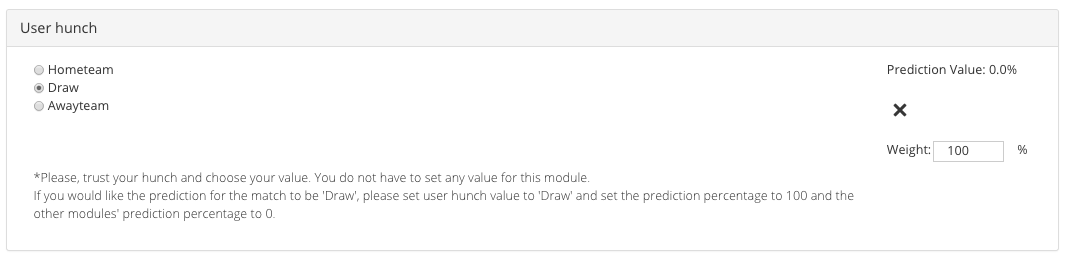
\includegraphics[width=.90\textwidth]{impl/images/userHunch}
		\caption{Module User Hunch.} \label{fig:using:userHunch}
	\end{center}
\end{figure}

The overall prediction is displayed underneath all modules, in a separate panel.

\begin{figure}[H]
	\begin{center}
		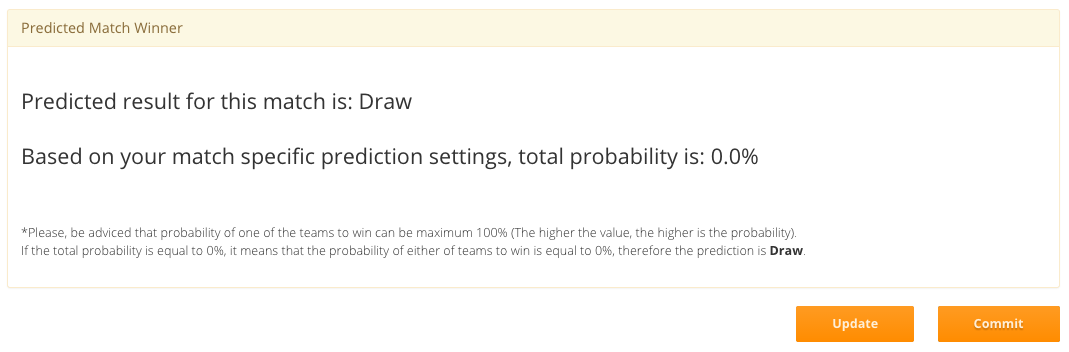
\includegraphics[width=.90\textwidth]{impl/images/prediction}
		\caption{Match result prediction.} \label{fig:using:prediction}
	\end{center}
\end{figure}

\subsubsection*{User journey}
\label{subsec:upcomingmatchviewuserjourney}
In the \textbf{read-only} mode the user can save the match to the dashboard by clicking "Save" button. 

In the \textbf{prediction} mode the user can update the prediction settings by overriding the current values in each of the input fields and pressing the button "Update" that is located at the bottom of the view. The overall prediction output will change every time the user updates the prediction settings or changes the hunch value. Once satisfied with the prediction outcome, the user can commit the match by pressing "Commit" button that is located next to "Update". Before the end of the match, the user can still navigate to the committed match view and see the all the details, including the prediction values, used weights and the final prediction. However, this time "Update" and "Commit" buttons will be disabled.

\begin{figure}[H]
	\begin{center}
		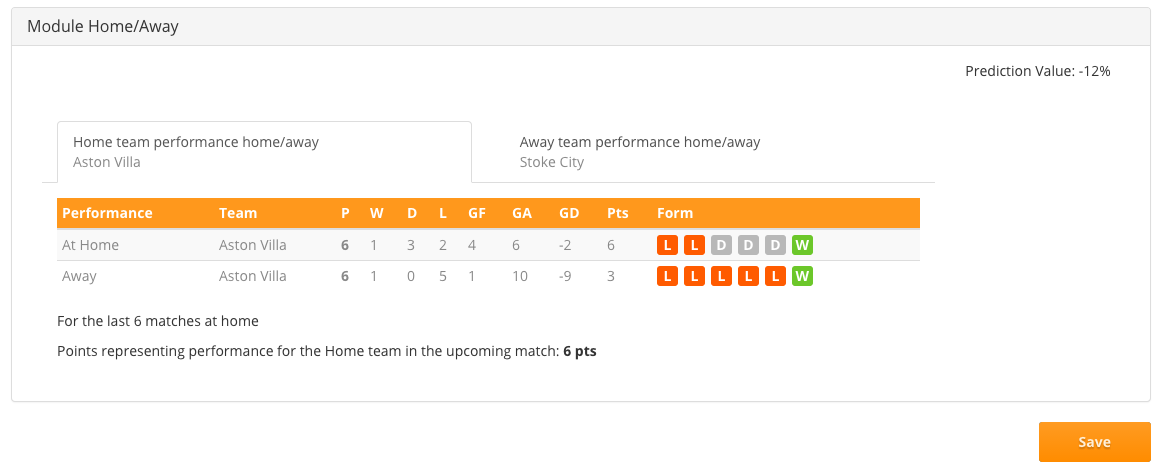
\includegraphics[width=.90\textwidth]{impl/images/matchoverviewex_from_main_page}
		\caption{An example of a prediction module in the Match Preview, user navigated from the main page.} \label{fig:using: matchoverviewex_from_main_page}
	\end{center}
\end{figure}

If the user comes to the upcoming match preview from the \emph{dashboard}, they will be able to see more information related to the actual result prediction and betting.
First of all, in each prediction module they will see an input fields for setting match specific prediction weights. Secondly, they will see a user hunch module. Finally, at the very bottom of the overview they will see calculated prediction result and two buttons - one to save the match specific settings and another to commit the bet.


most Explain how was implemented user hunch: combination of Flask Ajax and Sockets IO!!!
 
\subsection{Prediction}
\label{subsec:predictionimplementation}
After getting familiar with the \emph{Upcoming Match View}, the next logical step is to introduce the reader of this report to the Prediction feature of the application. This will aid understanding how to use the \emph{Upcoming Match View} and what kind of information this view offers to an intended user. The implementation of the Prediction feature was already explained in the chapter "Requirements Analysis", subsection "Prediction" \cite{subsec:prediction_requirements}. However, in this subsection I would like to outline the three levels of prediction settings used in the application, explain the calculation used behind each of the prediction values and also link the Prediction feature to other views. 

The application has three levels of prediction settings or weights. Firstly, the \emph{system default} prediction settings - a set of weights "recommended" to new users by the system. Once the user is registered with the application, they can set their own set of weights that will override the default settings, \emph{user default} prediction settings. This can be done through a "Prediction Settings" form, as explained in the subsection "Dashboard" \cite{subsec:dashboard}. From the moment those weights are saved in the database, they will apply to every newly saved match. The application also enables setting \emph {match specific} prediction settings that will only apply to one match. User can set match specific settings through the Upcoming Match view page.

There is a quite simple and logical equasions behind each of the prediction values that are displayed on the prediction modules panels and are used to calculate the overall match prediction. 
Equasions
An excel tables showing how the weighted average is calculated (check the hunch subsection, dont repeat yourself)

\subsection{Played Match View}
\label{subsec:playedmatchview}
User can navigate to this view by clicking the button "View match stats" on a panel representing a match that has already been played. Unlike the \emph{Upcoming Match View}, the \emph{Played Match View} looks the same to the users coming to this page both from their dashboards and from the matches overview page. 

The view contains already familiar match header, prediction statistics and a personalised feedback for the authenticated user. 

\begin{figure}[H]
	\begin{center}
		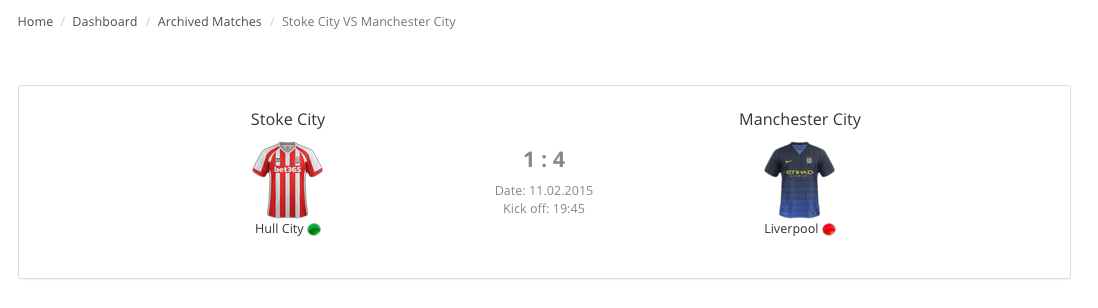
\includegraphics[width=.90\textwidth]{impl/images/matchHeader}
		\caption{Played Match View, match header.} \label{fig:matchheader}
	\end{center}
\end{figure}

Prediction statistics block contains information on the betting performance accross the SureThing users population with regards to this match. Stats contain the information on the number of users who saved the match to their dashboards, made a bet on the match, won or lost the bet. 

\begin{figure}[H]
	\begin{center}
		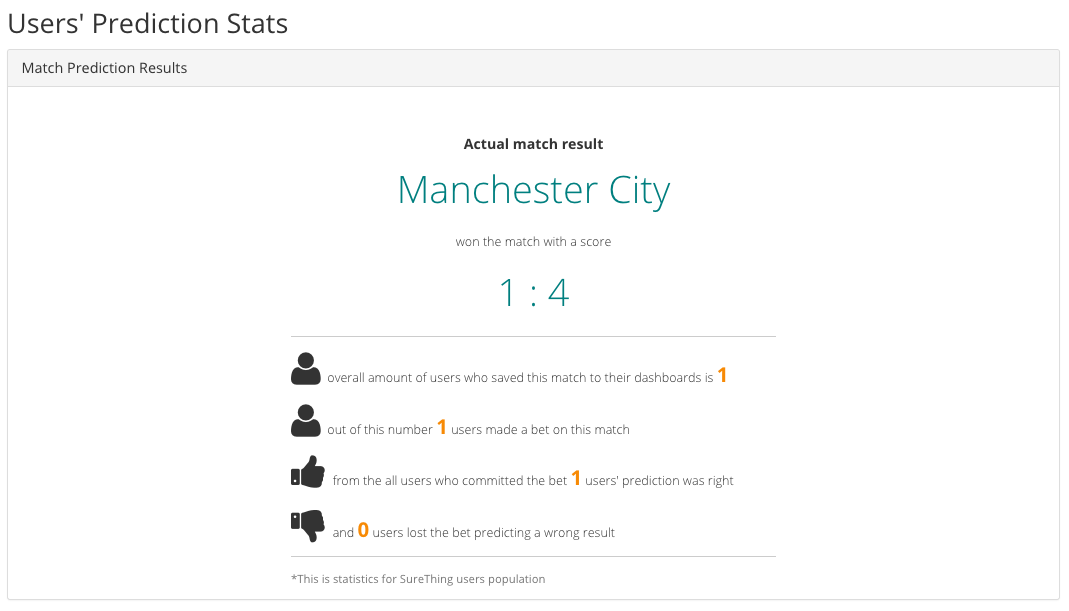
\includegraphics[width=.90\textwidth]{impl/images/predictionStats}
		\caption{Played Match View, users' prediction statistics.} \label{fig:predictionStats}
	\end{center}
\end{figure}

The view also offers a bar chart illustrating a breakdown of user preferences, namely how many users bet on "home", "draw" and "away" result.

\begin{figure}[H]
	\begin{center}
		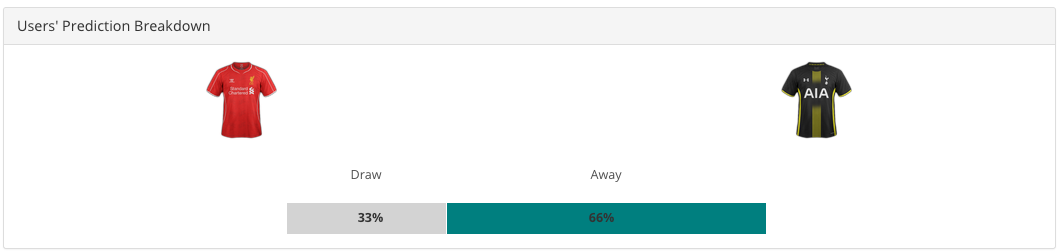
\includegraphics[width=.90\textwidth]{impl/images/predictionBreakdown}
		\caption{Prediction breakdown.} \label{fig:predictionBreakdown}
	\end{center}
\end{figure}

An authenticated user can also view a basic feedback indicating whether this particular user won or lost the bet.

\begin{figure}[H]
	\begin{center}
		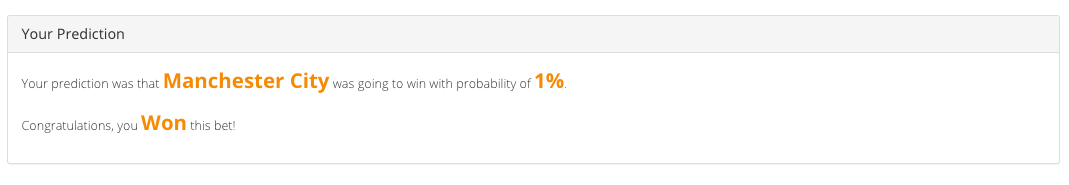
\includegraphics[width=.90\textwidth]{impl/images/feedback}
		\caption{Played Match View, feedback provided for authenticated users.} \label{fig:feedback}
	\end{center}
\end{figure}

\subsubsection*{User journey}
\label{subsec:playedmatchviewuserjourney}
The view is static and does not offer any additional interactions.

\subsection{Dashboard}
\label{subsec:dashboard}
SureThing dashboard is a centralised user space that provides convinient shortcuts to all the important prediction-related pages and tools. Dashboard can be used to store and view matches, change default prediction weights and make bets. It can be navigated to by clicking on item "Dashboard" in the navigation menu of the website, located at the top of the page. On navigating to the dashboard user can see a list of saved matches ordered by date and a \emph{dashboard menu} icon in the top left corner of the view. This is a screenshot of a typical dashboard view (only one match is saved):

\begin{figure}[H]
	\begin{center}
		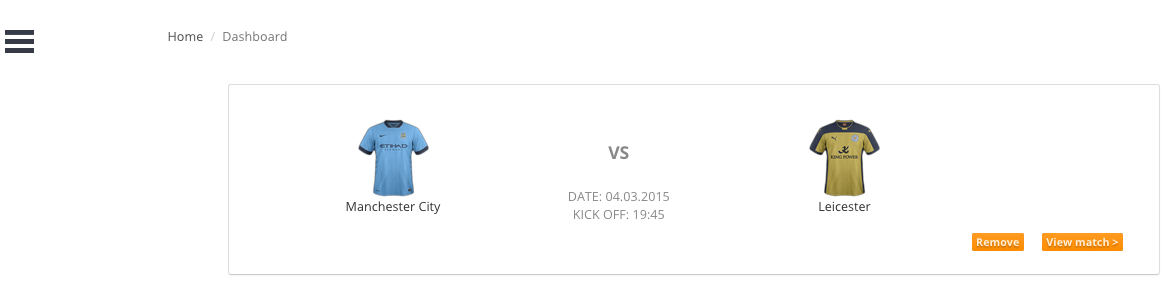
\includegraphics[width=.90\columnwidth]{impl/images/typicalDashboard}
		\caption{Dashboard view.} \label{fig:typicaldashboard}
	\end{center}
\end{figure}

Matches that already have been committed by the user have grey background and the predicted winner is highlighted. If the match has already been played, the result of the bet, either "Win" or "Loss" also appears on the match panel.

\begin{figure}[H]
	\begin{center}
		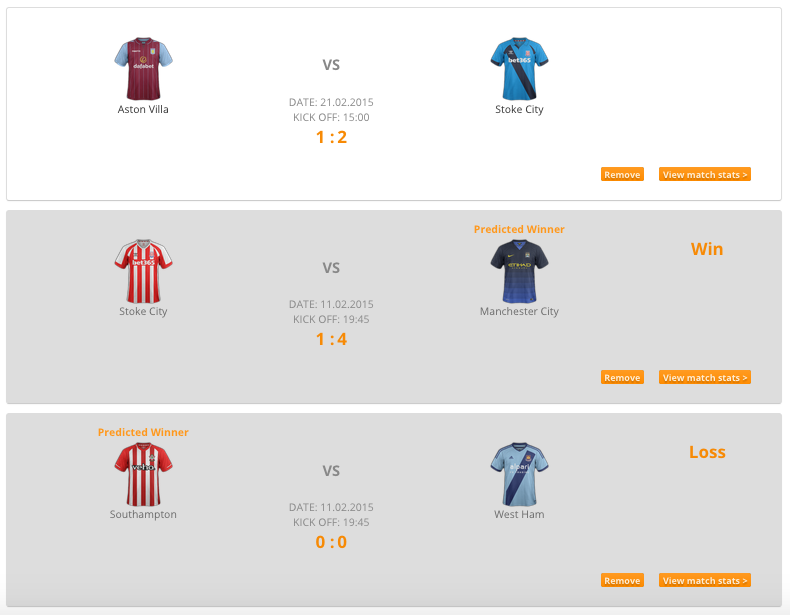
\includegraphics[width=.90\textwidth]{impl/images/dashboardCommittedMatches}
		\caption{An example of a Dashboard View with matches that have been committed and played.} \label{fig:dashboardcommittedmatches}
	\end{center}
\end{figure}

In case user does not have any matches saved, the dashboard looks as follows:

\begin{figure}[H]
	\begin{center}
		
\includegraphics[width=.90\textwidth]{impl/images/noSavedMatches}
		\caption{Dashboard with no saved matches.} \label{fig:using: nosavedmatches}
	\end{center}
\end{figure}

\subsubsection*{User journey}
\label{subsec:dashboarduserjourney}
In the top left corner user can see a small menu icon representing the dashboard menu. Clicking the button opens up the menu containing three items:

\begin{itemize}
	\item{Upcoming Matches. Displays all saved matches that have not been played yet. }
	\item{Archived Matches. Displays all saved matches that have already been played.}
	\item{Prediction Settings. A form that allows the user to set default prediction weights.}
\end{itemize}

A panel containing the dashboard menu slides in and covers part of the page. It can be easily dissmissed by choosing an item from the menu or clicking the "close" icon.

\begin{figure}[H]
	\begin{center}
		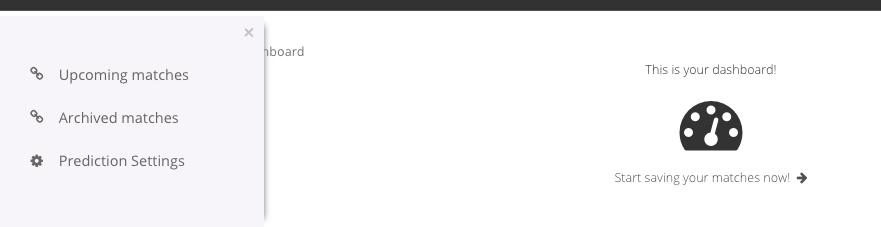
\includegraphics[width=.90\textwidth]{impl/images/dashboardMenu}
		\caption{Dashboard menu.} \label{fig:using: dashboardmenu}
	\end{center}
\end{figure}

If there no saved matches in the dashboard, user can navigate to the main pages containing upcoming events by clicking the link "Start saving your matches now >".

\subsection{Notifications}
\label{subsec:notifications}
This feature represents the one-way communication flow from SureThing to the application user. Every time a match previously commited by the user is finished (from the technical point of view, the match is changing its status to "played"), the application sends users messages notifying them whether their prediction guess was successfull. Such messages contain detailed information about the user prediction, as well as a link to the relevant \emph{Played Match View}.

\begin{figure}[H]
	\begin{center}
		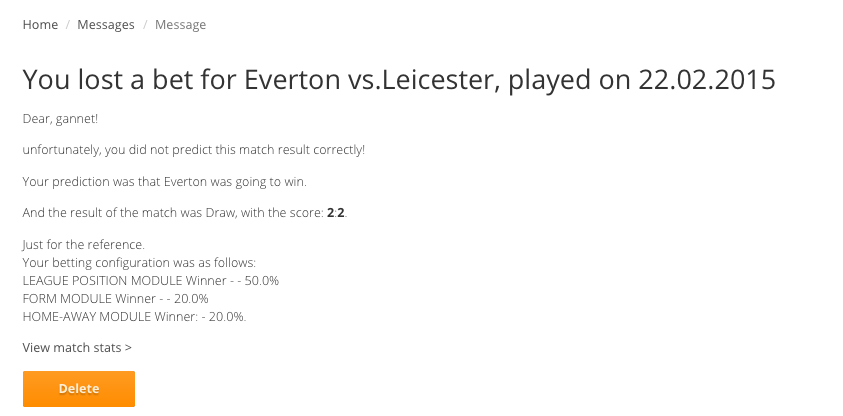
\includegraphics[width=.90\textwidth]{impl/images/message}
		\caption{An example of a message sent to the user.} \label{fig:using: message}
	\end{center}
\end{figure}

\subsubsection*{User journey}
\label{subsec:notificationsuserjourney}
Authenticated user can navigate to the notifications inbox by clicking at the envelope-shaped icon located on the right-hand side of the navigation menu. The orange colour of the icon in the screenshot below indicates that the inbox contains unread messages, otherwise the icon color is grey.

\begin{figure}[H]
	\begin{center}
		
\includegraphics[width=.90\textwidth]{impl/images/navigationMenu}
		\caption{Navigation menu panel with an inbox icon.} \label{fig:using: navigationmenu}
	\end{center}
\end{figure}

On clicking the icon user is taken to the notifications inbox. Unread messages are displayed in bold font.

\begin{figure}[H]
	\begin{center}
		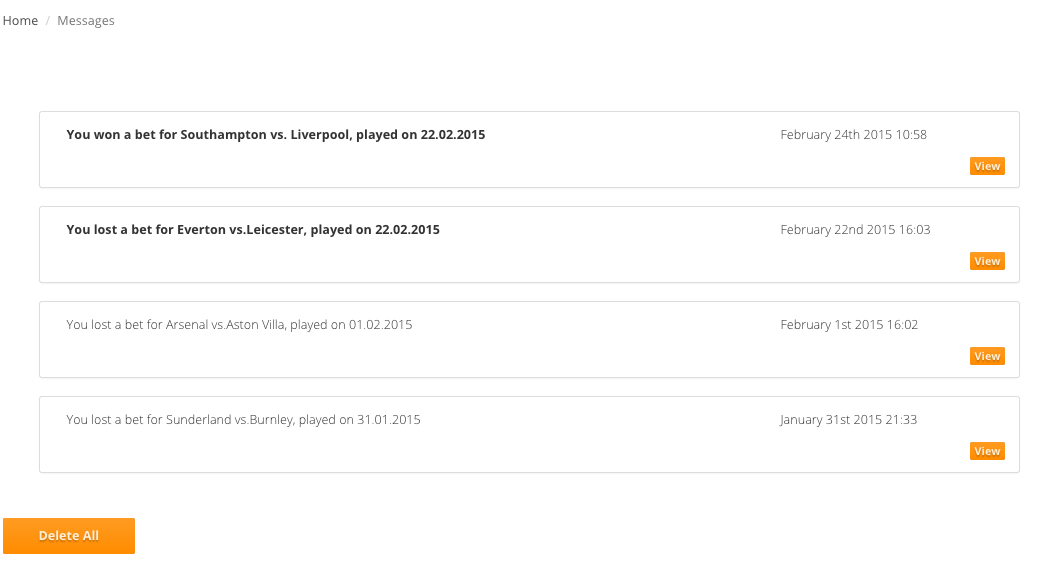
\includegraphics[width=.90\textwidth]{impl/images/inbox}
		\caption{User inbox.} \label{fig:using: inbox}
	\end{center}
\end{figure}

\subsection{Leaderboard}
\label{subsec:leaderboard}
Leaderboard is a view that contains a table capturing betting performance accross the population of the website. This page can be navigated to by clicking a "Leaderboard" entry in the navigation menu of the application. Each line of the Leaderboard table contains the most basic information about application users: usernames, location and their favourite team as well as the betting statistics: games committed, won and lost. The table is ordered by the amount of win points for each user. Thus, the winners are located on the top of the table. 

\begin{figure}[H]
	\begin{center}
		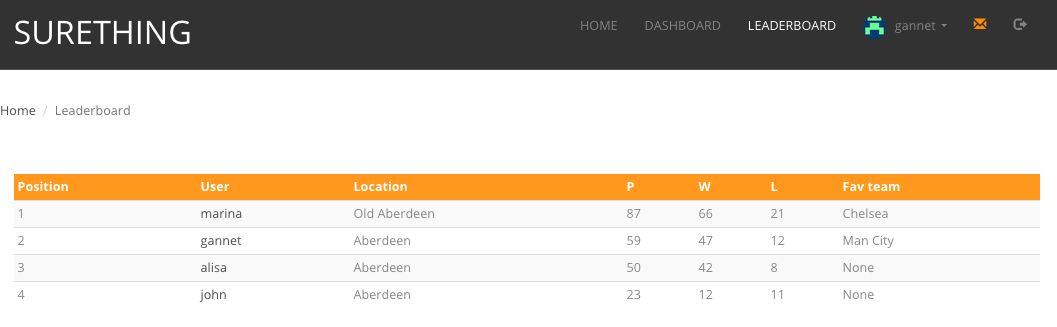
\includegraphics[width=.90\textwidth]{impl/images/leaderboard}
		\caption{Leaderboard.} \label{fig:using: leaderboard}
	\end{center}
\end{figure}

\subsubsection*{User Journey}
\label{subsec:leaderboarduserjourney}
Each username in the table is also a link. Clicking on the username of a user will take us to this user's profile page. Thus, an authenticated user can also view profiles of fellow users.

\section{Application Performance}
\label{sec:applicationperformance}
Performance is a very important aspect of a web application. DEF 

response time 

sockets, threads
multithreading
how I fixed performance on Match.update\_all\_matches

\section{Deploying the Application}
Cloud Deployment is the most recent trend in application hosting. The formal name of this technologu is Platform as a Service (PaaS).  In the PaaS model, a service provider offers a fully managed platform in which applications can run.

\section{Possible Future Enchancement}
\label{sec:enchancement}
The application can be further developed in many ways.  
When putting together the project requirements, a number of optional requirements were outlined. 

Although, one of the key features of the application is to try not to overhelm the user with statistics, as opposed to many football stats websites, this view would need a little bit more additional information to complete the big picture. 

\section{Conclusions}
The main conclusions for this chapter.
\chapter{Testing \& Evaluation}\label{ch:TestAndEval}
This chapter evaluates the overall project and provides results of tests carried out.

\section{Testing}
\subsection{Unit Testing}
The implementaion phase of the project was carried out in accordance with Agile Development. One of the cornerstones of Agile philosophy is Test Driven Development or TDD. The essense of TDD is to write the tests before even starting to write the production code . 

According to Miguel Grindberg \citep{book:Grindberg2014FlaskWebDevelopment}, "There are two very good reasons for writing unit tests. When implementing new functionality, unit tests are used to confirm that the new code is working in the expected way. ... A second, more important reason is that each time the application is modified, all the unit tests built around it can be executed to ensure that there are no regressions  in the existing code; in other words, that the new changes did not affect the way the older code works."

 For this project it was especially important to provide good tests coverage for the business logic behind the model layer and the external service layer of the application \ref{sec:applicationarchitecture_impl}. SureThing has a suite of unit tests that can be run anytime to validate the full functionality of the application.

Tests in this project are performed using Python \emph{unittest} library. 

\subsection{Continuous Integration with Travis CI}
As the application grows, it may become to take too long to run the unit tests. Therefore, it is worth automating this process by setting up a "Continuous Integration" or CI server. As a CI server was chosen Travis CI being easy to set up and available for free as a part of the GitHub Student Developer Pack. 
The service takes care of the unit testing allowing the developer to focus purely on the development process. Travis builds are triggered automatically when developer checks in the project code into the GitHub repository. Intergating Travis CI was just a matter of creation a configuration file, travis.yml. 

\begin{figure}[H]
	\begin{center}
		\includegraphics[width=.60\linewidth,natwidth=610,natheight=540]{eval/images/travisYml}
		\caption{Travis CI configuration file.} \label{fig:using:travisyml}
\end{center}
	
A Travis status icon indicating whether the tests passed or failed was embedded into the README file. This is a convinient feature that helped to keep an eye on the build status from the GitHub repository.

\end{figure}\begin{figure}[H]
	\begin{center}
		\includegraphics[width=.90\linewidth,natwidth=610,natheight=642]{eval/images/travisBadge}
		\caption{An extract from README on GitHub. Travis status icon indicates that the last build passed.} \label{fig:using:travisbadge}
	\end{center}
\end{figure}

\subsection{System Testing}


System Testing – This will test the system as a whole. This will be run by the developer taking into account the users requirements. Test cases will be created from the requirements with the inputs and expected outputs noted before the testing starts. Some of the test cases may satisfy more than one of the requirements. The tests will be carried out via the black box testing technique.

\subsection{User Acceptance Testing}
%Юзабилити-тестирование — это всегда вызов для разработчика. Для тестирования нужно предусмотреть и прописать все сценарии взаимодействия: %как пользователь будет себя вести, куда будет нажимать и попадать, что мы должны получить от пользователей (чтобы понять, соответствует ли %результат нашим ожиданиям).

\section{Evaluation and Future Development}
From my point of view, the project was successful. I started with zero knowledge of Python and now I feel that I would be able to use it on an industrial level. The project also made me realise the importance of Test Driven Development, as the application has complicated business logic in the background and good test coverage was a must to ensure smooth development process. The Acceptance Testing allowed me to get valuable user feedback and alter the design/navigation accordingly. In general, I am very pleased with the result and will continue to develop the application further.

The application has a lot of potential for improvement.
\chapter{Conclusion and Evaluation}
\label{ch:ConclusionEvaluation}
This chapter summarises the main outcomes and conclusions resulting from this body of work.

\section{Evaluation}
\label{sec:evaluation_conclusion}
Say something like "Based on the results from the evaluation and the general feedback from users, the application is amazing blah blah"

MAIN POINTS:
- this section has to answer the question: did we satisfy the objectives stated in the introduction? did we manage to do everything stated 
in the initial specification (chapter requirements)
- say smth like: this project was successfull, because
a) project aim was fullfilled (I developed an application useful for gamblers...balha blah)
b) almost all requirements that were outline initially were fullfilled (you need to look through the requirements and see if I did not implement some of the mandatory requirements and then mention it, say something like - this requirement was not implemented, as it was not important at this time or due to the time constraints)
c)  user acceptance tests had very good results - almost no issues
d) the application design was highly praised by the early users of the application

Overall, I feel the project has been very successful with a well-designed web application as a result.

The application has a lot of potential for improvement.

\section{Personal Statement}
\label{sec:personalstatement_conclusion}
project management issues - separate ability to give attention to the project, mentioned how it was incorporated into the studies, family. what have i learned, evaluating my performance, pm skills, technical skills, what things did i enjoy doing as part of the project. (put it in conclusion)

Discussion on how the project was managed. What things impacted the success of the project. How does the continually revised versions of the project plan compare to the initial draft developed at the start of the project. Did everything run according the schedule. Did elements such as exams \& coursework have any impact. 

As for the professional development, From my point of view, the project was successful. I started with zero knowledge of Python and now I feel that I would be able to use it on an industrial level. The project also made me realise the importance of Test Driven Development, as the application has complicated business logic in the background and good test coverage was a must to ensure smooth development process. The Acceptance Testing allowed me to get valuable user feedback and alter the design/navigation accordingly. In general, I am very pleased with the result and will continue to develop the application further.

\section{Improvements and Future Work}
\label{sec:enchancement_conclusion}
At the moment the developed application is a prototype suggesting what the system is capable of, rather than a fully-functional and well-tested application. 
There are many ways in which SureThing can be developed in the future. For example, it can remain a self-contained game and become a replacement to the real-world gambling experience. Another option is to link the application with the actual bookmakers and to turn it into a professional gambler's tool used that would provide all the relevant statistics and odds comparison.

The application can be further developed in many ways.  
When putting together the project requirements, a number of optional requirements were outlined. The optional requirements are basically the ways how the application can be further developed. More tests (check with potential users) would be required

Although, one of the key features of the application is to try not to overhelm the user with statistics, as opposed to many football stats websites, this view would need a little bit more additional information to complete the big picture. 


 I believe my project does hold commercial promise
 
 I hope that, through the module, I can at least develop a plausible promise as to what the system is capable of. The current implementation is a prototype, a placeholder… 
 
 If I were to continue with the project beyond university, my plan would be to develop even more cool features! May the odds be in your favour, username!


\appendix
\chapter{Target Audience Questionnaire}
\label{ch:ta_questionnaire_appendix}
The questionnaire presented below was answered by 9 respondents with strong interest in football betting. 

\section{Questions}
\label{sec:ta_questions_appendix}
This questionnaire intends to collect information about the way football punters make their betting decisions (decide which team to bet on).

The questionnaire should only take around five minutes to fill in and your answers will be used to aid the development of a web application simulating the football betting experience. The future application will provide its users with all the necessary football statistics (without going too much into detail) and allow them to participate in the prediction process by making their own prediction formula. 

\textbf{Question 1}\par
\textbf{How many times a week do you bet on football or other sporting events?}
\begin{itemize}
	\item Less than once a week
	\item 1 time a week
	\item 2-3 times a week
 	\item More than 3 times a week
 \end{itemize}
 
\textbf{Question 2}\par
\textbf{How many sources of information (websites, newspapers, your favourite mobile app) do you look into before making your placing your bet?}\par
\emph{For example, if you use 2 different websites (such as BBC News and Whoscored.com), the answer is 2.}
 \begin{itemize}
 	\item None
 	\item 2-3 sources
 	\item More than 3 sources
 \end{itemize}
 
\textbf{Question 3}\par
\textbf{Please specify the sources of information that you use to support your decision.}
 \begin{itemize}
	 \item TV programmes
	 \item Sports info websites (e.g., BBC News, The Guardian)
	 \item Football info websites (e.g., whoscored.com, squawka.com)
	 \item Gambling websites (e.g., Bet365, Ladbrokes)
	 \item Betting communities or forums (e.g.,OLGB.com)
	 \item Social Networks (e.g., betting tips from football experts on Twitter)
	 \item Printed media (newspapers)
	 \item Friend's advice
	 \item Mobile apps
	 \item Specify your own: 
\end{itemize}
  
\textbf{Question 4}\par
\textbf{What main factors do you take into account before placing a bet?}\par
\emph{Choose more than one or add your own}
 \begin{itemize}
	 \item Form
	 \item League position
	 \item Result of the previous match for each team
	 \item Home/Away performance so far in the season
     \item Change of a team manager
     \item Injuries/suspensions of players
	 \item Weather
	 \item Own hunch
	 \item Specify your own: 
\end{itemize}
 
\textbf{Question 5}\par
\textbf{Do you record your betting performance?}
\begin{itemize} 
 \item Yes
 \item No
\end{itemize}

\textbf{Question 6}\par
\textbf{What statement describes you best?}
 \begin{itemize}
 	\item I only use one bookmaker to place my bets
	\item I compare the odds several bookmakers and choose the best bookmaker for each match
\end{itemize}
 
\textbf{Question 7}\par
\textbf{Would you find a web application allowing you to participate in the prediction of a match result by making up you own prediction formula useful?}
\begin{itemize}
	\item Yes
	\item No
	\item Not sure
 \end{itemize}
 
\section{Answers}
\label{sec:ta_answers_appendix}
\noindent
\begin{sidewaystable}
\begin{tabular}{
  |p{\dimexpr.1\linewidth-2\tabcolsep-1.3333\arrayrulewidth}% column 1
  |p{\dimexpr.2\linewidth-2\tabcolsep-1.3333\arrayrulewidth}% column 2
  |p{\dimexpr.2\linewidth-2\tabcolsep-1.3333\arrayrulewidth}% column 3
  |p{\dimexpr.5\linewidth-2\tabcolsep-1.3333\arrayrulewidth}|% column 4
  }
  \hline
  \centering Respondent  & \centering Question 1  & \centering Question 2 & \centering\arraybackslash Question 3   \\ \hline
  1 & 1 time a week & 2-3 sources & Sports info websites (e.g., BBC News, The Guardian), Football info websites (e.g., whoscored.com, squawka.com) \\ \hline
  2 & Less than once a week & 2-3 sources & TV programmes, Printed media (newspapers) \\ \hline
  3 & 2-3 times a week & 2-3 sources & TV programmes, Printed media (newspapers), Friends advice \\ \hline
  4 & More than 3 times a week & More than 3 sources & TV programmes, Sports info websites (e.g., BBC News, The Guardian), Gambling websites (e.g., Bet365, Ladbrokes), Betting communities or forums (e.g.,OLGB.com), Social Networks (e.g., betting tips from football experts on Twitter), Mobile apps \\ \hline
  5 & More than 3 times a week & 2-3 sources & TV programmes, Gambling websites (e.g., Bet365, Ladbrokes), Printed media (newspapers) \\ \hline
  6 & Less than once a week & 2-3 sources & Football info websites (e.g., whoscored.com, squawka.com) \\ \hline
  7 & More than 3 times a week & 2-3 sources & Football info websites (e.g., whoscored.com, squawka.com), Gambling websites (e.g., Bet365, Ladbrokes), Mobile apps \\ \hline
  8 & Less than once a week & 2-3 sources & TV programmes, Sports info websites (e.g., BBC News, The Guardian), Printed media (newspapers) \\ \hline
  9 & 2-3 times a week & 2-3 sources & Sports info websites (e.g., BBC News, The Guardian) \\ \hline
\end{tabular}
\\[10pt]
\caption{Table illustrating answers to questions 1-3 in the Target Audience Questionnaire}
\end{sidewaystable}

\noindent
\begin{sidewaystable}
\begin{tabular}{
  |p{\dimexpr.1\linewidth-2\tabcolsep-1.3333\arrayrulewidth}% column 1
  |p{\dimexpr.3\linewidth-2\tabcolsep-1.3333\arrayrulewidth}% column 2
  |p{\dimexpr.1\linewidth-2\tabcolsep-1.3333\arrayrulewidth}% column 3
  |p{\dimexpr.4\linewidth-2\tabcolsep-1.3333\arrayrulewidth}% column 4
  |p{\dimexpr.1\linewidth-2\tabcolsep-1.3333\arrayrulewidth}|% column 5
  }
  \hline
  \centering Respondent  & \centering Question 4  & \centering Question 5 &  \centering Question 6 & \centering\arraybackslash Question 7   \\ \hline
  1  & Form, League position, Result of the previous match for each team, Own hunch & No & I only one bookmaker to place my bets & Yes \\ \hline
  2 & Form, League position, Injuries/suspensions of players & No & I only use one bookmaker to place my bets & Not sure \\ \hline
  3 & Form, League position, Home/Away performance so far in the season, Own hunch & No & I compare the odds several bookmakers and choose the best bookmaker for each match & Yes \\ \hline
  4  & Form, League position, Result of the previous match for each team, Home/Away performance so far in the season, Own hunch & No & I only use one bookmaker to place my bets & Yes \\ \hline
   5 & Form, League position, Home/Away performance so far in the season, Change of a team manager & No & I compare the odds several bookmakers and choose the best bookmaker for each match & Yes \\ \hline
   6 & Form, Own hunch & No & I only use one bookmaker to place my bets & No \\ \hline
   7 & Form, Home/Away performance so far in the season, Injuries/suspensions of players & No & I only use one bookmaker to place my bets & Yes \\ \hline 
   8 & Form, League position, Result of the previous match for each team, Injuries/suspensions of players, Own hunch & No & I only use one bookmaker to place my bets & Yes \\ \hline
   9 & Form, Own hunch, Whether or not the odds appear to offer good value & No & I only use one bookmaker to place my bets & Yes \\ \hline
  \end{tabular}
 \caption{Table illustrating answers to questions 4-7 in the Target Audience Questionnaire}

\end{sidewaystable}


\chapter{User Acceptance Questionnaire}
\label{ch:ua_questionnaire_appendix}
The questionnaire presented below was answered by 7 potential end users. 

\section{Questions}
\label{sec:ua_questions_appendix}
This questionnaire intends to verify that the developed website is easy to understand and use for the potential users.

Please, complete the following steps using the application: 

\begin{enumerate}
   \item Create a new account 
   \item Login 
   \item Look through the list of matches and choose the ones you are the most interested in, then save them to dashboard
   \item Set your own prediction weights 
   \item Commit to betting on a match
\end{enumerate}

On completing the steps, please answer the following questions:

\textbf{Question 1}\par
\textbf{Which step did you find the most difficult to carry out and why?}\par
\emph{Please, provide your own answer.}
 
\textbf{Question 2}\par
\textbf{How easy was it to set up a new account?}\par
\emph{Please, rate the following question on a scale of 1 (Very easy) to 10:  (Very confusing).}
 
\textbf{Question 3}\par
\textbf{Was it easy to find and set the prediction settings?}\par
 \emph{Please, rate the following question on a scale of 1 (Very easy) to 10:  (Very confusing).}
  
\textbf{Question 4}\par
\textbf{How would you rate the overall user friendliness of the application?}\par
 \emph{Please, rate the following question on a scale of 1 (Very easy) to 10:  (Very confusing). }
 
 \textbf{Question 5}\par
\textbf{Did you find there was enough statistics to aid your decision making, and if not, what would you want to see?}\par
\emph{Please, provide your own answer.}
 
 \textbf{Question 6}\par
\textbf{What did you find was the best aspect of the application? E.g., design, navigation}\par
\emph{Please, provide your own answer.}

\textbf{Question 7}\par
\textbf{What did you find was the worst aspect of the application?}\par
\emph{Please, provide your own answer.}

\textbf{Question 8}\par
\textbf{What would you like to see in the application?}\par
\emph{Please, provide your own answer.}

\section{Answers}
\label{sec:ua_answers_appendix}

\noindent
\begin{sidewaystable}
\begin{tabular}{
  |p{\dimexpr.1\linewidth-2\tabcolsep-1.3333\arrayrulewidth}% column 1
  |p{\dimexpr.4\linewidth-2\tabcolsep-1.3333\arrayrulewidth}% column 2
  |p{\dimexpr.3\linewidth-2\tabcolsep-1.3333\arrayrulewidth}% column 3
  |p{\dimexpr.1\linewidth-2\tabcolsep-1.3333\arrayrulewidth}% column 4
  |p{\dimexpr.1\linewidth-2\tabcolsep-1.3333\arrayrulewidth}|% column 5
  }
  \hline
  \centering Respondent  & \centering Question 1  & \centering Question 2 &  \centering Question 3 & \centering\arraybackslash Question 4   \\ \hline
  1  & Probably the changing the prediction settings but even that wasn't hard really & More leagues & 10 & 8 \\ \hline
  2 & Saving matches to the dashboard, wasn't immediately apparent why I had to do that & A way to communicate with friends using the same app, maybe a separate league table for friends than just for all users & 9 & 7 \\ \hline
 3 & Committing the match, it wasn't immediately apparent that I can only commit a match previously saved in the dashboard & Maybe some news feeds & 7 & 8 \\ \hline
  4 &  Changing the prediction settings, it could have been clearer what I was supposed to do & A help menu or FAQ would be useful & 7 & 6 \\ \hline
  5 &  It was all fairly easy & More leagues, comparison betting odds from different bookies & 10 & 10 \\ \hline
  6 &  Saving matches to the dashboard, wasn't sure why I had to do that & More social interaction, link to Facebook & 8 & 7 \\ \hline
  7 &  Setting the prediction weights, wasn't sure of what to set them to so I juts left them at their default settings & A guide to how to use the app would have been nice & 10 & 7 \\ \hline

  \end{tabular}
 \caption{Table illustrating answers to questions 1-4 in the User Acceptance Questionnaire}

\end{sidewaystable}

\noindent
\begin{sidewaystable}
\begin{tabular}{
  |p{\dimexpr.1\linewidth-2\tabcolsep-1.3333\arrayrulewidth}% column 1
  |p{\dimexpr.1\linewidth-2\tabcolsep-1.3333\arrayrulewidth}% column 2
  |p{\dimexpr.3\linewidth-2\tabcolsep-1.3333\arrayrulewidth}% column 3
  |p{\dimexpr.3\linewidth-2\tabcolsep-1.3333\arrayrulewidth}% column 4
  |p{\dimexpr.2\linewidth-2\tabcolsep-1.3333\arrayrulewidth}|% column 5
  }
  \hline
  \centering Respondent  & \centering Question 5  & \centering Question 6 &  \centering Question 7 & \centering\arraybackslash Question 8   \\ \hline
  1  & 8 & The layout was easy on the eye and simple enough to find your way about & Not enough football leagues represented & Yes \\ \hline
  2 & 5 & The design was simple but nice to look at & The dashboard seems a but pointless & Yes \\ \hline
  3 & 8 & The prediction feature was great, especially because I could change it myself & The design was a little boring & Yes \\ \hline
  4 & 5 & The way the stats and matches were presented, very clear & The way to change the prediction settings could have been explained better & Yes \\ \hline
  5 &  10 & It was very self explanatory how it all worked together & Lack of football leagues to use & No, betting odds \\ \hline
  6 &  7 & I liked the design & The dashboard wasn't very useful & Yes \\ \hline
  7 &  5 &  Navigating from page to page was easy & I was confused about the prediction settings & Yes \\ \hline

  \end{tabular}
 \caption{Table illustrating answers to questions 5-7 in the User Acceptance Questionnaire}

\end{sidewaystable}
 
\chapter{Installation Instructions}
\label{ch:install_appendix}
The code can be checked out using git by executing the following command in the terminal:

\noindent See the following command :
\begin{lstlisting}[language=bash]
  $ git clone git@github.com:marinamarina/sure-thing.git
\end{lstlisting}

Installation instructions are found at the following url:

\url{https://www.github.com:marinamarina/sure-thing/blob/master/README.md}.


If any issues arise regarding installation of any part of the system, do not hesitate to contact me at 1014481@rgu.ac.uk

\chapter{Credits}
\label{ch:credits_appendix}
Some the application's code was taken from the GitHub repository accompanying the book by Miguel Grindberg "Flask Web Development" \citep{book:Grindberg2014FlaskWebDevelopment}. Below are listed the components of the system that rely on this code to some extent:

\begin{itemize}
	\item user authentication, account verification
	\item basic test suite
	\item user authentication test suite
\end{itemize}

Some of the handy decorator functions used in the Python code were taken from Flask documentation \citep{documentation:Flask}, section "View Decorators".

\chapter{Project Management}
\label{ch:pm_appendix}
The project was not developed following a single software development methodology. Different techniques from various methodologies were used for the project. Some of the planning was made beforehand in the traditional, Waterfall approach fashion, such as researching the project background, defining application requirements, sketching the application wireframes, etc. On the other hand, some of the design techniques were adopted from the Agile methodology, namely user journeys. 

The project implementation phase was carried out in an iterative manner. For defining the project requirements, the application functionality was divided into clearly defined units (so called "high-level features" introduced in the chapter "Requirements Analysis" \ref{ch:requirementanalysis}), each associated with an implementation iteration. Excel sheets were used for defining the set of tasks for each iteration. GitHub issue tracker was also used as a supporting productivity tool for this project. Code related tasks were recorded as "issues" for the project GitHub repository. In general, the GitHub issue tracker was a very efficient tool for keeping the project organised. 

\chapter{Presentation Slides}
\label{ch:slides_appendix}
The following is a weekly summary of the work carried during the development of this body of work. It covers tasks that were completed, tutorials that were worked through, articles that were read and reviews of discussions / meetings held with the project supervisor and other third parties. 






\nocite{*}
\bibliographystyle{plainnat}
\bibliography{shchukina-2015-surething}
\end{document}
